\documentclass[12pt,oneside,a4paper,parskip]{scrbook}
\usepackage[utf8]{inputenc}
\usepackage{csquotes}
\usepackage[ngerman]{babel}
\usepackage{floatflt}
\usepackage{subfigure}
\usepackage[pdftex]{graphicx}
\graphicspath{ {./pictures/} }
\usepackage[hidelinks]{hyperref}
\usepackage[german]{cleveref}
\usepackage{color}
\usepackage{amssymb}
\usepackage{textcomp}
\usepackage{nicefrac}
\usepackage{scrhack}
\usepackage{pdfpages}
\usepackage{float}
\usepackage{pdflscape}
\usepackage{subfigure}
\usepackage{pdfpages}
\usepackage[verbose]{placeins}
\usepackage[nouppercase,headsepline,plainfootsepline]{scrlayer-scrpage}
\usepackage{listings}
\usepackage{xcolor}
\usepackage{color}
\usepackage{caption}
\usepackage{subfigure}
\usepackage{epstopdf}
\usepackage{longtable}
\usepackage{setspace}
\usepackage{booktabs}
\usepackage[style=numeric,backend=biber]{biblatex}
\bibliography{./thesis.bib}



%%%%%%%%%%%%%%%%%%%
%% definitions
%%%%%%%%%%%%%%%%%%%
\def\BaAuthor{Lennard Rose, Jochen Schmidt, Moritz Zeitler}
\def\BaAuthorStudyProgram{Informatik} %% Wirtschaftsinformatik, E-Commerce, Informationssysteme
\def\BaType{Projektarbeit} %% Masterarbeit
\def\BaTitle{Entwicklung einer Data Mining Plattform f\"ur Corona Daten}
\def\BaSupervisorOne{Prof. Rott}
\def\BaSupervisorTwo{Prof. Fertig}
\def\BaDeadline{\today}

\ifdefined\iswithfullname
  \def\ShowBaAuthor{\BaAuthor}
\else
  \def\ShowBaAuthor{N.~N.}
\fi

\hypersetup{
pdfauthor={\ShowBaAuthor},
pdftitle={\BaTitle},
pdfsubject={Subject},
pdfkeywords={Keywords}
}

%%%%%%%%%%%%%%%%%%%
%% configs to include
%%%%%%%%%%%%%%%%%%%
\colorlet{punct}{red!60!black}
\definecolor{background}{HTML}{EEEEEE}
\definecolor{delim}{RGB}{20,105,176}
\colorlet{numb}{magenta!60!black}

\definecolor{gray}{rgb}{0.4,0.4,0.4}
\definecolor{darkblue}{rgb}{0.0,0.0,0.6}
\definecolor{cyan}{rgb}{0.0,0.6,0.6}

\definecolor{pblue}{rgb}{0.13,0.13,1}
\definecolor{pgreen}{rgb}{0,0.5,0}
\definecolor{pred}{rgb}{0.9,0,0}
\definecolor{pgrey}{rgb}{0.46,0.45,0.48}

\definecolor{maroon}{cmyk}{0, 0.87, 0.68, 0.32}
\definecolor{halfgray}{gray}{0.55}
\definecolor{ipython_frame}{RGB}{207, 207, 207}
\definecolor{ipython_bg}{RGB}{247, 247, 247}
\definecolor{ipython_red}{RGB}{186, 33, 33}
\definecolor{ipython_green}{RGB}{0, 128, 0}
\definecolor{ipython_cyan}{RGB}{64, 128, 128}
\definecolor{ipython_purple}{RGB}{170, 34, 255}

\lstset{
  basicstyle=\ttfamily,
  columns=fullflexible,
  showstringspaces=false,
  commentstyle=\color{gray}\upshape
  linewidth=\textwidth
}

\lstdefinelanguage{json}{
    basicstyle=\normalfont\ttfamily,
    numbers=left,
    numberstyle=\scriptsize,
    stepnumber=1,
    numbersep=8pt,
    showstringspaces=false,
    breaklines=true,
    backgroundcolor=\color{background},
    literate=
     *{0}{{{\color{numb}0}}}{1}
      {1}{{{\color{numb}1}}}{1}
      {2}{{{\color{numb}2}}}{1}
      {3}{{{\color{numb}3}}}{1}
      {4}{{{\color{numb}4}}}{1}
      {5}{{{\color{numb}5}}}{1}
      {6}{{{\color{numb}6}}}{1}
      {7}{{{\color{numb}7}}}{1}
      {8}{{{\color{numb}8}}}{1}
      {9}{{{\color{numb}9}}}{1}
      {:}{{{\color{punct}{:}}}}{1}
      {,}{{{\color{punct}{,}}}}{1}
      {\{}{{{\color{delim}{\{}}}}{1}
      {\}}{{{\color{delim}{\}}}}}{1}
      {[}{{{\color{delim}{[}}}}{1}
      {]}{{{\color{delim}{]}}}}{1},
}



\lstset{language=xml,
  morestring=[b]",
  morestring=[s]{>}{<},
  morecomment=[s]{<?}{?>},
  stringstyle=\color{black},
  numbers=left,
  numberstyle=\scriptsize,
  stepnumber=1,
  numbersep=8pt,
  identifierstyle=\color{darkblue},
  keywordstyle=\color{cyan},
  backgroundcolor=\color{background},
  morekeywords={xmlns,version,type}% list your attributes here
}

\lstset{language=Java,
  showspaces=false,
  showtabs=false,
  tabsize=4,
  breaklines=true,
  keepspaces=true,
  numbers=left,
  numberstyle=\scriptsize,
  stepnumber=1,
  numbersep=8pt,
  showstringspaces=false,
  breakatwhitespace=true,
  commentstyle=\color{pgreen},
  keywordstyle=\color{pblue},
  stringstyle=\color{pred},
  basicstyle=\ttfamily,
  backgroundcolor=\color{background},
%  moredelim=[il][\textcolor{pgrey}]{$$},
%  moredelim=[is][\textcolor{pgrey}]{\%\%}{\%\%}
}

\newcommand*{\forcetwosidetitle}[1][1]{%
 \begingroup
   \cleardoubleoddpage
   \KOMAoptions{titlepage=true}% useful e.g. for scrartcl
   \csname @twosidetrue\endcsname
   \maketitle[{#1}]
 \endgroup
}


\begin{document}


%%%%%%%%%%%%%%%%%%%
%% Titelseite
%%%%%%%%%%%%%%%%%%%


\frontmatter
\titlehead{%  {\centering Seitenkopf}
  {Hochschule für angewandte Wissenschaften Würzburg-Schweinfurt\\
   Fakultät Informatik und Wirtschaftsinformatik}}
\subject{\BaType}
\title{\BaTitle\\[15mm]}
\subtitle{\normalsize{vorgelegt an der Hochschule f\"{u}r angewandte Wissenschaften W\"{u}rzburg-Schweinfurt in der Fakult\"{a}t Informatik und Wirtschaftsinformatik zum Abschluss eines Studiums im Studiengang \BaAuthorStudyProgram}}
\author{\ShowBaAuthor}
\date{\normalsize{Eingereicht am: \BaDeadline}}
\publishers{\
  \normalsize{Erstpr\"{u}fer: \BaSupervisorOne}\\
  \normalsize{Zweitpr\"{u}fer: \BaSupervisorTwo}\\
}
\forcetwosidetitle


%%%%%%%%%%%%%%%%%%%
%% abstract
%%%%%%%%%%%%%%%%%%%

\section*{Zusammenfassung}

TODO

\section*{Abstract}

TODO

\chapter*{Danksagung}



%%%%%%%%%%%%%%%%%%%
%% Inhaltsverzeichnis
%%%%%%%%%%%%%%%%%%%
\tableofcontents



%%%%%%%%%%%%%%%%%%%
%% Main part of the thesis
%%%%%%%%%%%%%%%%%%%
\mainmatter

\chapter{Einführung und Motivation}\label{ch:intro}
Wir in unserem Team, bestehend aus Jochen Schmidt, Lennard Rose und Moritz Zeitler hatten nach unserem Gemeinsamen Programmierprojekt beschlossen, wieder zusammen zu arbeiten und diesmal in eine ganz andere Richtung zu gehen. Hierzu muss man wissen, dass unser Programmierprojekt damals aus einem Multiplayer-Computerspiel bestand, welches wir ausschließlich mit C++ sowie SDL programmierten. Da wir nichts vorgefertigtes an Code oder Lösungen benutzten und alles "von der Pike auf"  entwickelten, lag der Fokus vor allem auf Algorithmen, Datenstrukturen und Patterns. Auch wenn uns diese Art des Entwickelns allen sehr Spaß gemacht hat und unser Projekt sehr Erfolgreich war, wollten wir mit dieser Projektarbeit nochmal in eine ganz andere Richtung gehen um uns als Entwickler weiter zu entwickeln und unserem Repertoire ein paar neue Tools hinzuzufügen. Mit dem Thema Datamining war für uns auch sehr schnell ein Thema gefunden, Coronadaten boten sich aus aktuellem Anlass an und da Moritz noch ein paar alte Rechner im Keller stehen hatte, beschlossen wir nicht nur eine Lösung, sondern ein betriebsbereites System zu entwickeln. \newline
Der Fokus dieser Projektarbeit soll also ganz klar auf Schnittstellen, Interaktionen und Recherche über Lösungsmöglichkeiten liegen.

\chapter{Entwicklungsprozess}
Beim Entwicklungsprozess wurde sich f\"ur eine scrumartige L\"osung entschieden. So werden klassische Artefakte und Tools wie etwa das Daily oder der Backlog entsprechend angepasst angewandt. Anpassung meist im Sinne der zeitlichen Komponente. Da das Projekt parallel w\"ahrend des Semesters abl\"auft wurde hier das 'Daily', von einem t\"aglichen auf einen w\"ochentlichen Rhythmus umgestellt. Das Backlog wird durch das Team selbst bef\"ullt da es keinen 'Product Owner' gibt. Genauso wurden die Sprints abgewandelt, durch die zeitliche Entzerrung wird hier direkt auf eine dynamische Sprintl\"ange gesetzt die jeweils zum Sprint-Anfang abgestimmt worden ist. \newline
G\"anzlich verzichtet wurde auf die Sprint Retrospektive, zwar hat sich im Laufe des Projekts der Prozess dynamisch angepasst, allerdings wurde hier nicht explizit ein Artefakt bzw. Termin durchgef\"uhrt. \"Anderungen am Prozess wurden kurzfristig und in direkter Absprache mit allen Teammitgliedern beschlossen. Vereinfachend hinzu kam, dass sich die Projektaufgaben durch die vielen, verschiedenartigen Scraper, welche nicht weiter miteinander interagieren, gut aufteilen ließen. So konnte jeder sein Tempo selbst bestimmen und es waren wenig zusätzliche Maßnahmen nötig um die Arbeit an gemeinsam genutzten Modulen zu koordinieren.

\chapter{Projektmanagement}
\section{Risikoanalyse}
Für unser Projekt haben wir nach der generellen Planung des Aufbaus und Systems eine Risikoanalyse vorgenommen. Da wir auf viele verschiedene heterogene Elemente angewiesen sind war es uns wichtig uns vorher eine Übersicht möglicher Risiken zu erstellen. Für unsere Bewertung haben wir uns auf die Kategorien {gering, mittel und hoch} festgelegt für die Wahrscheinlichkeit des Eintritts und die Größe des Schadens bei Eintritt.
\subsection{Risikoidentifikation}
Wir haben folgende Risiken erfasst:

\begin{itemize}
\item\textbf{Ausfall von Hardwareteilen}
Da wir bei unserer Hardware auf unsere privaten ehemaligen genutzten Rechner setzen und damit auf heterogene Systeme und keine wirklichen Servern ist durchaus davon auszugehen das der ein oder andere Ausfall der Hardwareteile während des Projekts möglich ist. Das führt je nach schwere des Schadens bis zu einem Ausfall eines Nodes.
\item\textbf{Ausfall ganzer Nodes}
Da wir wie bereits erwähnt auf unterschiedliche Hardware setzten und hierbei bereits ein Risiko besteht es könnte ein schwerwiegenden Ausfall geben kommt aber auch noch hinzu das anderweitig z.B. durch falsche Konfiguration ein Ausfall entstehen kann.
\item\textbf{Inkompatibilität von Python Versionen zwischen Windows und Ubuntu}
Wir führen alle unsere Entwicklungen auf Windows durch und für die Server setzen wir auf eine etwas ältere Ubuntu Version. Dadurch sehen wir es als Risiko beim späteren deployen unserer Skripte auf den Servern.
\item\textbf{Inkompatibilität von Frameworks zueinander}
Für das Scheduling, das Dateisystem etc. setzen wir auf viele verschiedene Frameworks die alle Hand in Hand gehen müssen. Da sehen wir ein direktes Risiko von Inkompatibiltät
\item\textbf{Schaden an der Festplatte durch Transport}
Dadurch das die Rechner nicht fest bei einem Projektmitglied oder festgelegtem Ort während der Entwicklung standen und des öfteren zwischen einander
transportiert wurden war die Unversehrtheit des Systems sowie vor allem der HDDs ein Risiko. Die Rechner sollten erst im späteren Verlauf in der FHWS eingesetzt werden.
\end{itemize}
\subsection{Risikobewertung}
%-> Tabelle
Ausfall von Hardwareteilen - Häufigkeit: mittel; Schaden: gering
Ausfall eines Nodes - Häufigkeit: gering; Schaden: hoch
Inkompatibilität zwischen Windows/Ubuntu - Häufigkeit: hoch; Schaden: mittel
Inkompatibilität zwischen Frameworks - Häufigkeit: hoch; Schaden: gering
Transportschäden - Häufigkeit: mittel; Schaden: mittel
\subsection{Risikomatrix}
\begin{figure}[h!]
\caption{Risikomatrix}
\label{risikoMatrix}
\centering
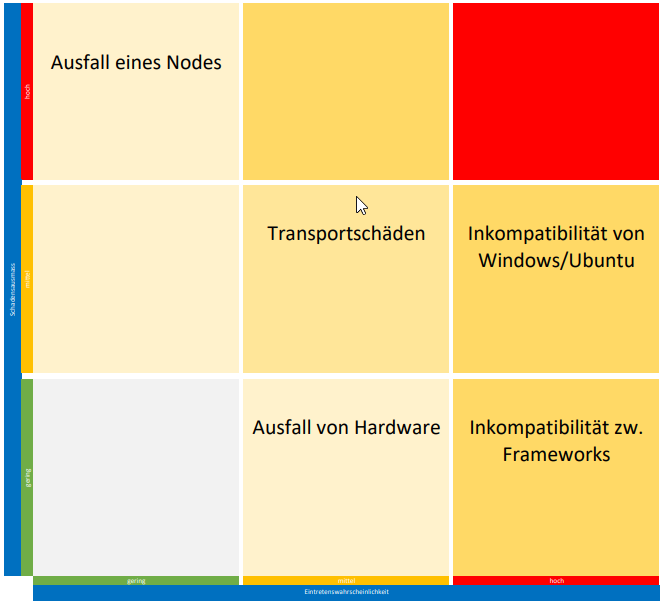
\includegraphics[scale=1.0]{pictures/risikoanalyse.png}
\end{figure}


\chapter{Cluster Technologien}
Grunds\"atzlich wird das komplette Projekt auf Basis eines Hadoop Cluster erstellt. Hadoop ist ein Framework f\"ur skalierbare und verteilt arbeitende Software. Gerne wird auch der Begriff  Hadoop \"Okosystem verwendet da es einen kompletten Zoo von Technologien (z.B. Zookeeper, HBase, Flink, Storm, Pig, Solr) gibt die im Hadoop Umfeld verwendet werden kann. Hadoop erm\"oglicht eine horizontale Skalierung, dies bedeutet das dem System dynamisch zus\"atzliche Knoten, angeh\"angt werden k\"onnen die dann die Rechenleistung, bzw die Speicherkapazit\"at des Clusters erh\"ohen. In der Basis besteht Hadoop aus YARN und dem HDFS die zusammen mit dem MapReduce Konzept eine Datenverarbeitung erm\"oglichen. Zus\"atzlich zu diesen Standardkomponenten wurden noch Apache Oozie sowie Apache Zeppelin installiert. Diese einzelnen Konzepte sowie zus\"atzliche Basisinformationen zum Cluster werden im folgenden noch genauer erkl\"art.

\section{YARN}
YARN steht f\"ur 'Yet another resource negotiater'. Die Aufgabe des YARN darin die verf\"ugbaren Ressourcen auf alle anfallenden Aufgaben zu verteilen. Dies bedeutet YARN ist 'Resourcemanager' als auch 'Job-Scheduler'.
\begin{figure}[H]
	\centering
	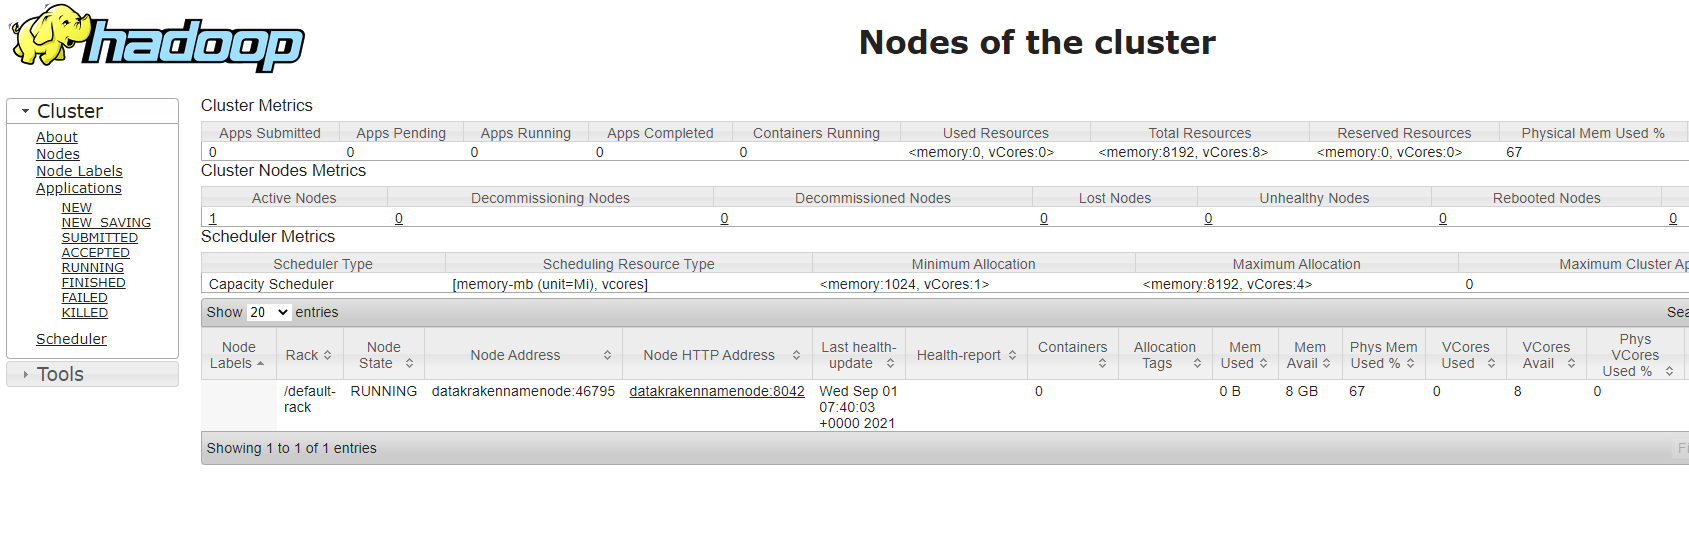
\includegraphics[scale=0.3]{yarnClusterOverview.png}
	\captionsetup{justification=centering}
	\caption{\"Ubersichtsseite von YARN}
	\label{pic:yarnClusterOverview}
\end{figure}
Bevor YARN zu seinem Namen kam wurde der Dienst zun\"achst 'MapReduce2' genannt. Jedoch entwickelte sich YARN dann schnell dahingehend das auch noch andere Aufgaben neben MapReduce, wie zum Beispiel interaktive Abfragen oder Echtzeit-Analysen von Streaming-Daten, ausgef\"uhrt werden k\"onnen, was dazuf\"uhrte die Verbindung zu MapReduce im Namen aufzul\"osen. \newline
Die tats\"achliche grundlegende Idee hinter der Funktion von YARN ist das Aufspalten von 'ResourceManager' und 'ApplicationMaster'. Der ResourceManager ist die zentrale Komponente mit dem der User in Kommunikation steht oder besser gesagt mit dem eine Anfrage an Rechenkapazit\"at kommuniziert. F\"ur eine solche Anfrage erstellt der 'ResourceManager' einen enstprechenden 'ApplicationMaster', dieser k\"ummert sich dann von Anfang bis Ende um diesen einen Auftrag. Status, Neustart oder Fehlerbehandlung werden komplett von ihm \"ubernommen der 'ResourceManager' hat damit nichts mehr zu tun. Der 'ApplicationMaster' \"ubergibt seine Aufgabe an einen Nodemanager der dann die tatsa\"achliche Ausf\"uhrung startet, bzw eine Container entgegen nimmt und diesen ausf\"uhrt. Die \"Uberwachung dieses Containers ist allerdings wiederum, wie bereits erw\"ahnt, Aufgabe des 'ApplicationMaster'. Nach Abschluss der Ausf\"uhrung meldet sich der 'ApplicationMaster' wieder beim 'ResourceManager' ab und gibt seine Ressourcen wieder frei.\cite{Shenoy.2014}
\begin{figure}[H]
	\centering
	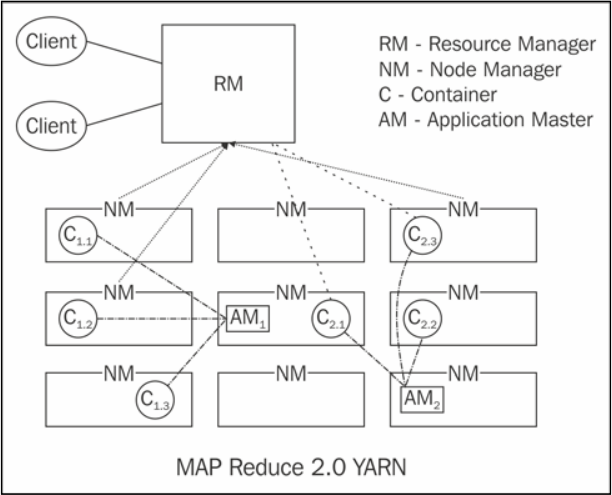
\includegraphics[scale=0.9]{yarnOverview.png}
	\captionsetup{justification=centering}
	\caption{Visualisierung der Aus\"uhrung eines YARN-Containers}
	\label{pic:yarnOverview}
\end{figure}
Dies ist an dieser Stelle wahrscheinlich durchaus unverst\"andlich, was allerdings f\"ur den nachfolgenden Bericht nicht all zu relevant ist.
\newline An dieser Stelle ist es wichtig zu erw\"ahnen das die Auftr\"age die von YARN ausgef\"uhrt werden immer in Containern ausgef\"uhrt werden, vergleichbar mit Docker oder Kubernetes. Dies bedeutet das alle Abh\"angigkeiten mit in den Container geliefert werden m\"ussen. Außerdem ist zu beachten das es teilweise zu Problemen mit Netzwerk bzw. Internetzugriff kommen kann.

\section{HDFS}
Das 'Hadoop Distributed File System' ist die Technologie, die im Hadoop Umfeld die verteilte Datenablage erm\"oglicht. HDFS hat viele Gemeinsamkeiten zu andern bekannten verteilten Dateisystemen wie zum Beispiel Amazon S3. Der Hauptunterschied zu den meisten Technologien ist Widerstandsf\"ahigkeit gegen\"uber Fehlern. Der Grundsatz von Hadoop war immer das ein Cluster aus Standard bzw. Kosteng\"unstiger Hardware aufgebaut werden kann, was allerdings zu einer h\"oheren Fehleranf\"alligkeit f\"uhren kann. Das HDFS wurde in diesem Zusammenhang nach dem Grundsatz entwickelt das es immer ein Teil der Hardware nicht funktioniert.\cite{hdfsFailure} \newline
Mit unter der wichtigste Grundsatz ist aber wahrscheinlich dass, wenn m\"oglich, nicht die Daten zum Prozess bewegt werden sondern der Code bzw. der Algorithmus zu den Daten gebracht wird.\cite{movingComputation} Je gr\"oßer der Datensatz desto gr\"oßer die Kosten diese Daten zu verschieben. Und da sich im Normalfall ein 'BigData' System haupts\"achlich um große Datenmengen k\"ummert wird dieser Prozess genau umgedreht, der Algorithmus kommt zu den Daten. Die n\"otigen Voraussetzungen und Schnittstellen stellt das HDFS zur Verf\"ugung um Applikationen es zu erm\"oglichen diese Idee umzusetzen.

\section{Oozie und Cron}  \label{ooziecron}
Als Grundprinzip sollen alle Daten kontinuierlich und automatisch im Cluster gespeichert werden. Hierzu m\"ussen die entsprechenden Datensammler regelm\"assig gestartet werden oder dauerhaft als Daemon laufen. In diesem Projekt wurde davon abgesehen dauerhaft laufende Datensammler zu verwenden, da diese grunds\"atzlich Rechenkapazit\"at binden. Dies widerspricht dem Prinzip, dass Hadoop individuell Rechenkapazit\"at zur Verf\"ugung stellt.\newline
Als Alternative gibt es im Hadoop-Technologie-Zoo bereits eine L\"osung die es erm\"oglicht zeitlich, oder sogar daten-getriggert, automatisch Aufgaben zu starten - Apache Oozie. Eigentliche Hauptaufgabe von Oozie sind die sogenannten 'Workflows', was nichts anderes ist als ein vordefinierter Arbeitsablauf. Um zeitlich gesteuerte Aufgaben zu starten gibt es die sogenannten 'Coordinator Jobs', sie sind vergleichbar mit den normalen Workflows und sind einzelne, konfigurierbare Arbeitsschritte. Wichtig ist an dieser Stelle zu wissen, dass unabh\"angig von der Aufgabe, egal ob Python Script, MapReduce oder Email-Action, immer ein Art Container (vergleichbar mit Docker) erstellt wird, der dann von YARN ausgef\"uhrt wird. \newline
Die logische Konsequenz daraus ist, dass dem auszuf\"uhrenden Paket bzw. Container alle n\"otigen Abh\"angigkeiten mitzugeben sind. Dies bedeutet zum Beispiel, dass alle Python Libraries mit in das auszuf\"uhrende Paket mit eingebunden sein m\"ussen. F\"ur fast alle Datensammler stellt dies kein Problem dar, lediglich der Scraper, der sich um die Corona-Massnahmen k\"ummert, stellt ein großes Problem dar. Mit Tesseract nutzt der Scraper ein Commandline-Tool das nicht mit ein ausf\"uhrbares Paket gepackt werden kann. \newline
Deswegen musste als Alternative Cron verwendet werden, was ebenso zeitlich gesteuert Scripte ausf\"uhren kann. Genauer wird an dieser Stelle nicht auf Cron eingegangen, da es sich hier um eine mehr als nur bekannte Standardkomponente des Unix-Kernel handelt. Problematisch ist hier leider das die Scripte nicht \"uber YARN sondern \"uber einen Knoten selbst ausgef\"uhrt werden. Von Vorteil ist hier aber das sowohl der Installationsaufwand quasi nicht vorhanden ist und sich auch das Paketieren der Software bedeutend einfacher darstellt als bei Oozie.

\section{Zeppelin}
Um die gesammelten Daten auch effektiv verarbeiten zu k\"onnen, muss ein geeigneter Prozess aufgezeigt werden. Das Grundkonzept von Hadoop ist immer noch MapReduce. Dies funktioniert im Entwicklungsprozess immer indem ein Job programmiert wird und dann auf dem Cluster getestet wird. F\"ur Testzwecke ist das ein großer Aufwand. Heutzutage geht daher  der Trend hin zu RapidPrototyping-Umgebungen. So gibt es auch im Hadoop Umfeld eine entsprechende Option, Apache Zeppelin. Zeppelin ist stark vergleichbar mit JupyterHub und ist somit eine RapidProtoyping-Umgebung mit User Management. Innerhalb der sogenannten Notebooks kann fast jede erdenkliche Programmiersprache als Interpreter verwendet werden (z.B. Python, Java, R, Elasticsearch, hive, spark). Der grosse Vorteil von Zeppelin gegen\"uber Jupyter ist, dass der Kernel (Programmiersprachen spezifischer Prozess der Code ausf\"uhrt) auf YARN ausgef\"uhrt werden kann und somit auf alle Ressourcen des Cluster zugreifen kann.
\begin{figure}[H]
	\centering
	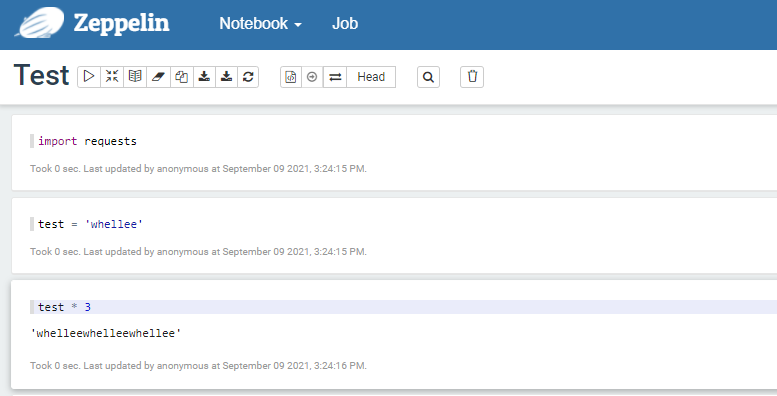
\includegraphics[scale=0.6]{zeppelinOverview.png}
	\captionsetup{justification=centering}
	\caption{\"Ubersicht Zeppelin Oberfl\"ache}
	\label{pic:zeppelinOverview}
\end{figure}
\chapter{Datenablagekonzept}
F\"ur die Datenablage wurde zun\"achst ein entsprechendes Konzept entwickelt. Dieses Konzept basiert auf den Daten die abgelegt werden sollen. Hierzu wird zun\"achst ein \"Uberblick \"uber die zu ablegenden Daten gegeben:
\begin{itemize}
	\item Corona Nachrichten/Artikel
	\item Corona RKI Daten
	\item Corona Maßnahmen
	\item Wetterdaten
\end{itemize}
Jede einzelne Datenquelle wird nun genauer beleuchtet und ein entsprechendes Datenablagekonzept erarbeitet. Da die Konzepte sich aber sehr \"ahneln wird der Hauptteil der Erkl\"arung bei der gr\"ossten Komponente den Corona-Artikeln zu finden sein. Grunds\"atzlich werden alle Daten sowohl in Elasticsearch als auch im HDFS abgelegt. Wobei das HDFS haupts\"achlich f\"ur Data Governance Zwecke genutzt wird. Bedeutet das hier die Rohdaten unver\"andert gespeichert werden sollen um sp\"ater immer noch Zugriff auf die Original Daten zu haben, was eine Art 'sanity-check' der Daten erm\"oglicht.
\section{Corona Nachrichten/Artikel}
Die Corona Nachrichten bzw. Artikel werden in zwei unterschiedlichen Technologien abgelegt. Zun\"achst betrachten wir die Rohdaten. Wie bereits erkl\"art wird jeder Artikel in Rohformat gespeichert. Diese Daten sind aber f\"ur die Auswertung und zur \"Ubersicht der Datensammlung erst mal unwichtig. Dies bedeutet das diese Daten nicht in einer Datenbank indiziert, sondern nur im HDFS abgelegt werden. Die Geschwindigkeit des HDFS f\"ur den Datenzugriff ist ausreichend um die Daten bei einer genauen Auswertung ad-hoc zu lesen. Streng genommen k\"onnte man sogar argumentieren dass das HDFS nichts anderes als ein 'key-value store' ist. So wird im Hintergrund eine Datei die unter einem gewissen Pfad abgelegt worden ist f\"ur den User als klassischer Dateipfad angezeigt (Ordner durch 'forward-slashes' getrennt und am Ende des Pfades ein Dateiname), intern aber der Pfad einen key darstellt. Dies ist n\"otig um die Verteilung und Ausfallsicherheit der Daten \"uber mehrere Knoten gew\"ahrleisten zu k\"onnen. Allerdings ist dies f\"ur den User faktisch nicht bemerkbar, da dieser immer mit den entsprechenden Pfaden arbeitet.
Um nun den Kreis zu schliessen werden nicht nur Meta-Daten der Artikel gespeichert sondern auch der komplette Artikel im Rohformat um Datenverlust vorzubeugen und die Konsistenz der Daten sp\"ater noch pr\"ufen zu k\"onnen. Die Rohdaten werden dann abgelegt unter dem Pfad: '/datakraken/articles/region/quelle/zeitung/Datum/'. Dieser Pfad wird dann zu den Meta-Daten hinzugef\"ugt. Der Titel der Dateien im Textformat selbst setzt sich aus region + quellenname + artikeltitel zusammen. \newline
 Meta-Daten werden vom entsprechenden Scraper parallel zu den Rohdaten erzeugt. Dies Daten werden dann, unter entsprechendem Index Namen im Elasticsearch Cluster abgelegt. Dies hilft dabei eine \"Ubersicht über die Daten und deren Inhalt zu erhalten, einen Status zu bekommen in welchem Ma?e die Daten in das System kommen und erm\"oglicht eine rudiment\"are Analyse. Die Daten setzen sich zusammen aus den Atributen der Quelle: Name, Region und URL, des entsprechenden Artikels: URL, Titel, Datum der Veröffentlichung, Autor, Typ, Beschreibung und Stichworten, sowie Daten zur Erzeugung: Indizierungs bzw. Erstellungszeitpunkt, Dateiname und Pfad.
\section{Corona RKI Daten}
Die wichtigsten Basis Informationen \"uber den Status der Corona-Pandemie in Deutschland sind h\"ochst wahrscheinlich Inzidenz-Wert und Impfquote. Diese Informationen werden in diesem Projekt \"uber das Robert-Koch-Institut bezogen. \"Uber eine \"offentliche API kann nicht nur Inzidenzwert pro Bundesland, sondern auch per Bezirk bezogen werden. Ausserdem sind alle Informationen zum derzeitigen Impfstand in Deutschland, sowie Informationen zu PCR- und Schnelltests in Deutschland verf\"ugbar. Alle Informationen die hier von der API zur Verf\"ugung gestellt werden, werden auch gespeichert. Hier folgt der Scraper dem Allgemeinen Konzept, die Original Daten werden im HDFS abgelegt und dann mit minimaler Ver\"anderung im Elasticsearch indiziert.
\section{Corona Maßnahmen}
Das soeben erw\"ahnte Konzept der Nachrichten wird genauso f\"ur die Massnahmen verwendet. Rohdaten werden im HDFS abgelegt, w\"ahrend die beschreibenden Daten im Elasticsearch indiziert werden. Diese Massnahmen werden mit folgendem Pattern abgelegt: '/datakraken/measures/\$bundesland\$/\$Datum\$+\$TimeStamp\$/'.
\section{Wetterdaten}
Auch die Wetterdaten werden im gleichen Stil abgelegt. Heisst die einzelnen Wetterlogs werden als Dokumente im Elasticsearch abgelegt und auch hier\"uber abgefragt. Allerdings werden die Wetterdaten auch noch entsprechend des allgmeinen Konzepts im HDFS abgelegt. Die Ablage Struktur im HDFS ist in folgendem Pattern:  '/datakraken/weather/\$Stadt\$/\$Datum\$/\$TimeStamp\$'.
\section{'Querdenker' Telegram Gruppen}
Im Bereich der Telegram Gruppen muss hier differenziert werden. Die verschickten Nachrichten an sich werden mit den Meta-Daten zusammen im Elasticsearch abgelegt. H\"angt allerdings an der Nachricht noch eine Datei ein, oder ein Link, wird die Datei im HDFS abgelegt. Dazu wird eine Referenz erstellt und mit im Elasticsearch abgelegt. Die Ablage Struktur im HDFS ist in folgendem Pattern: '/datakraken/telegram/\$GruppenName\$/\$Datum\$/\$NachrichtId\$\_\$TimeStamp\$'.

\chapter{Cluster und Deployment}
%mehr so braindump, überarbeiten%
\section{Überblick} Bereits bei der Ideenfindung zu unserer Projektarbeit hatten wir uns dazu entschieden, nicht nur den Quellcode für den Datensammler zu schreiben, sondern das ganze auch auf einem Cluster zum laufen zu bringen. Hierfür haben wir 3 alte Rechner (Bis zur Explosion eines Netzteils ursprünglich 4) von Moritz genommen. Die Absicht hier war aus alter, ungenutzter Hardware neuen Wert zu schöpfen und Tieferen Einblick in Serververwaltung mit Linux zu erhalten. Wir haben bei dem Aufsetzen der Nodes mit der benötigten Software bewusst von der Verwendung von Docker abgesehen, trotz des Wissens, dass es die einfachste Möglichkeit gewesen wäre. Grund ist, dass wir dieses Projekt vornehmlich dazu nutzen wollen, ein breites Fundament an Wissen aufzubauen, welches auch Serveradministration beinhalten soll. Um Elasticsearch mit Docker zu starten, ist nicht viel mehr nötig als sich ein Compose-File aus dem Internet zu suchen und zu starten.

\section{Betriebssystem} Als Betriebssystem wählten wir Ubuntu 18.04 LTS, da es mit ca. einem Drittel aller Linuxserver das meistverwendete Betriebssystem darstellt. Als Bezeichnung für die einzelnen Knoten wählten wir 'datakrakennamenode', für den Masternode, sowie 'datanodekraken1' und 'datanodekraken2', für die beiden Anderen. Auf jedem Knoten legten wir einen User mit Namen 'hadoop' an. Im laufe des Projekts stellte sich heraus, dass eine 'sauberere' Lösung gewesen wäre, einen User zu allgemeinen Serververwaltung, sowie jeweils einen User zum laufen der Elasticsearch sowie Hadoop Daemons zu erstellen. Auch wurde der Fehler gemacht den Rootuser nur Stiefmütterlich zu behandeln und nicht mit Passwort einzurichten, dies kostete beim Recovery viel Zeit und nerven.\newline
Als nächsten Schritt wiesen wir allen Nodes statische private IP-Adressen zu, hierzu wählten wir die vom Router vergebenen Adressen. \pagebreak
\begin{lstlisting}[caption=datakrakennamenode: /etc/netplan/00-installer-config.yaml,label=hosts,language=bash]
network:
  ethernets:
    enp6s0:
      dhcp4: no
      dhcp6: no
      addresses: [192.168.0.115/24]
      gateway4: 192.168.0.1
      nameserver:
       addresses: [8.8.8.8,8.8.4.4]
  renderer:
   NetworkManager
  version: 2
#mit sudo netplan try/-apply anwenden!
\end{lstlisting}
Diese mapten wir auf die Knotennamen in der "hosts"- Datei, um sie bei der weiteren Konfiguration immer mit ihrem Namen angeben zu können.
\begin{lstlisting}[caption=etc/hosts,label=hosts,language=bash]
...
192.168.0.115 datakrakennamenode
192.168.0.103 datanodekraken1
192.168.0.201 datanodekraken2
...
\end{lstlisting}
Jeder Node erhielt ausserdem noch Java 8 zum ausführen von Hadoop bzw. Elasticsearch/Kibana, die Umgebungsvariable wurde gesetzt.
\begin{lstlisting}[caption=etc/environment,label=javaenv,language=bash]
JAVA_HOME=/usr/lib/jvm/java-8-openjdk-amd64
\end{lstlisting}

\section{Hadoop}
\subsection{Allgemeines}
Hadoop ist eine opensource Lösung von Apache, die parallele Verarbeitung und verteilte Datenhaltung auf einem Cluster möglich macht. Mit Hadoop ist auch immer das Hadoop Distributet File System (HDFS) sowie YARN, ein Framework zur Ablaufplanung von verteilten Anwendungen gemeint. \newline
Der Cluster besteht aus einem Master und vielen sogenannten Workernodes. Der Master behält dabei den Überblick über das verteilte Dateisystem. Dies tut er indem auf ihm 2 Daemons laufen, der Namenode und der Resourcemanager. Der Namenode managt das verteilte Dateisystem und weiß wo die gespeicherten Daten sind. Der Resourcemanager verwaltet YARN-Jobs und kümmert sich um die Planung und Ausführung von Prozessen auf den Workernodes. \newline
Workernodes hingegen sind zum speichern der Daten und dem Ausführen der Jobs da. Auch sie hosten zwei Daemons, den Datanode, zum verwalten der Daten auf dem Node, sowie dem Nodemanager, der die Ausführung der Tasks auf dem Node verwaltet.
\subsection{Setup}
Hadoop Version 3.2.2 wurde als Binary für Ubuntu heruntergeladen und entpackt. Der Einfachheit halber wurde der Ordner von "hadoop-3.2.2" zu "hadoop" umbenannt.
Als nächstes wurden die nötigen Umgebungsvariablen gesetzt und die PATH-Variable angepasst. %hier muss noch hin warum environment und nicht einfach .bashrc
\begin{lstlisting}[caption=etc/environment,label=env,language=bash]
HADOOP_HOME=/home/hadoop/hadoop
YARN_HOME=/home/hadoop/hadoop
HADOOP_COMMON_HOME=/home/hadoop/hadoop
HADOOP_HDFS_HOME=/home/hadoop/hadoop
HOME=/home/hadoop
PATH=/usr/local/sbin:/usr/local/bin:/usr/sbin:/usr/bin:/sbin:/bin:/usr/games:/usr/local/games:/snap/bin:/bin:/home/hadoop/hadoop/bin:/home/hadoop/hadoop/sbin:/usr/lib/jvm/java-8-openjdk-amd64/bin:/usr/lib/jvm/java-8-openjdk-amd64/sbin
\end{lstlisting}
Ausserdem wurden noch folgende Konfigurationen vorgenommen: \newline
\begin{lstlisting}[caption=/hadoop/etc/hadoop/core-site.xml,label=coresitexml,language=bash]
<configuration>
        <property>
            <name>fs.default.name</name>
            <value>hdfs://datakrakennamenode:9000</value>
        </property>
    </configuration>
\end{lstlisting}
\begin{lstlisting}[caption=hadoop/etc/hadoop/hdfs-site.xml,label=hdfssitexml,language=bash]
<configuration>
    <property>
            <name>dfs.namenode.name.dir</name>
            <value>/home/hadoop/data/nameNode</value>
    </property>

    <property>
            <name>dfs.datanode.data.dir</name>
            <value>/home/hadoop/data/dataNode</value>
    </property>

    <property>
            <name>dfs.replication</name>
            <value>1</value>
    </property>
</configuration>
\end{lstlisting}
\begin{lstlisting}[caption=hadoop/etc/hadoop/hdfs-site.xml,label=hdfssitexml,language=bash]
<configuration>
    <property>
            <name>dfs.namenode.name.dir</name>
            <value>/home/hadoop/data/nameNode</value>
    </property>

    <property>
            <name>dfs.datanode.data.dir</name>
            <value>/home/hadoop/data/dataNode</value>
    </property>

    <property>
            <name>dfs.replication</name>
            <value>1</value>
    </property>
</configuration>
\end{lstlisting}\begin{lstlisting}[caption=/hadoop/etc/hadoop/mapred-site.xml,label=mapredsitexml,language=bash]
<configuration>
    <property>
            <name>mapreduce.framework.name</name>
            <value>yarn</value>
    </property>
    <property>
            <name>yarn.app.mapreduce.am.env</name>
            <value>HADOOP_MAPRED_HOME=$HADOOP_HOME</value>
    </property>
    <property>
            <name>mapreduce.map.env</name>
            <value>HADOOP_MAPRED_HOME=$HADOOP_HOME</value>
    </property>
    <property>
            <name>mapreduce.reduce.env</name>
            <value>HADOOP_MAPRED_HOME=$HADOOP_HOME</value>
    </property>
</configuration>
\end{lstlisting}
\begin{lstlisting}[caption=/hadoop/etc/hadoop/yarn-site.xml,label=yarnsitexml,language=bash]
<configuration>
    <property>
            <name>yarn.acl.enable</name>
            <value>0</value>
    </property>

    <property>
            <name>yarn.resourcemanager.hostname</name>
            <value>datakrakennamenode</value>
    </property>

    <property>
            <name>yarn.nodemanager.aux-services</name>
            <value>mapreduce_shuffle</value>
    </property>
</configuration>

\end{lstlisting}
\begin{lstlisting}[caption=/hadoop/etc/hadoop/workers,label=workers,language=bash]
datanodekraken1
datanodekraken2
\end{lstlisting}
\begin{lstlisting}[caption=Formatieren des HDFS und Start/Stop,label=start,language=bash]
hdfs namenode -format
start-dfs.sh
stop-dfs.sh
\end{lstlisting}
\begin{lstlisting}[caption=Check ob daemon auf datakrakennamenode läuft,label=jpsnamenode,language=bash] %hier noch orginal von cmd einfügen
>jps
21922 Jps
21804 NameNode
21879 SecondaryNameNode
\end{lstlisting}
\begin{lstlisting}[caption=Check ob daemon auf den workern läuft,label=jpsworker,language=bash]
>jps
21912 Jps
21434 DataNode
\end{lstlisting}
Sollten die Daemons wider erwarten nicht anspringen, hat es sich als hilfreich erwiesen den tempordner von Hadoop zu löschen und das HDFS erneut zu formatieren.

\section{Elasticsearch}
Alles nach anleitung von elastic installiert.
Kibana nur auf datakrakennamenode installiert
User zu gruppen elasticsearch und kibana hinzugefügt
Berechtigungen über die verzeichnisse verteilt

\begin{lstlisting}[caption=elasticsearch.yml,label=elasticyml,language=bash]
cluster.name: datakraken
cluster.initial_master_nodes: ["datakrakennamenode"]
node.name: datakrakennamenode
node.master: true
path.data: /var/lib/elasticsearch
path.logs: /var/log/elasticsearch
discovery.zen.ping.unicast.hosts: ["datakrakennamenode", "datanodekraken1", "datanodekraken2"]
\end{lstlisting}

\begin{lstlisting}[caption=kibana.yml,label=kibanayml,language=bash]
server.port: 5601
server.host: "datakrakennamenode"
server.name: "datakraken"
elasticsearch.hosts: ["http://datakrakennamenode:9200"]
\end{lstlisting}


\begin{lstlisting}[caption=Setup zum automatischen Start mit jedem Boot, label=boot,language=bash]
sudo /bin/systemctl daemon-reload
sudo /bin/systemctl enable elasticsearch.service
#nur auf datakrakennamenode:
sudo /bin/systemctl enable kibana.service
\end{lstlisting}
\begin{lstlisting}[caption=Manuelles Starten/ Stoppen von Elasticsearch/Kibana,label=startstopelastic,language=bash]
sudo systemctl start elasticsearch.service
sudo systemctl stop elasticsearch.service
sudo systemctl start kibana.service
sudo systemctl stop kibana.service
\end{lstlisting}


\begin{lstlisting}[caption=Befehl zum durchsuchen der Logdaten,label=logelastic,language=bash]
sudo journalctl --unit elasticsearch --since  ">>heutiges datum<<"
\end{lstlisting}

\begin{lstlisting}[caption=Befehl zum durchsuchen der Logdaten,label=logkibana,language=bash]
journalctl -u kibana.service
\end{lstlisting}

\begin{lstlisting}[caption=Statusabfrage Elasticsearch,label=statuselastic,language=bash]
curl -XGET 'datakrakennamenode:9200/_cluster/health?pretty'
\end{lstlisting}

\begin{lstlisting}[caption=Statusabfrage Kibana,label=statuskibana,language=bash]
curl -XGET 'datakrakennamenode:5601/api/status'
curl -XGET 'datakrakennamenode:5601/status'
\end{lstlisting}

Über ssh beide mittels IP adresse abrufbar
%Braindump ende%

\chapter{Datenquellen}
\section{Nachrichtenartikel}
Die Onlinepräsenzen von Zeitungen sind Grundsätzlich sehr gut Organisiert. Artikel sind meist sehr übersichtlich in Themengebiete oder Dossiers unterteilt, lassen sich aber zur Not auch mittels allgegenwärtiger Suchfunktion gut vorfiltern. Auch URLs zu den einzelnen Artikeln sind meist in Themen und Regionsspezifische Pfade unterteilt und somit einfach zu filtern. Als Datenquelle wurden daher so gut wie möglich durch eben genannte Möglichkeiten zum Coronathema vorgefilterte Artikelübersichtsseiten verwendet deren Artikel anschließend über Regex-Zeichenfolgen in ihrer URL weiter gefiltert wurden. Als Quellen können neben den 32 vorkonfigurierten auch beliebig weitere Quellen verwendet werden, da der Scraper dafür ausgelegt wurde, von allen Zeitungsquellen zu jedem Thema Informationen speichern zu können. Bei den vorkonfigurierten Quellen handelt es sich um Zeitungsartikel über die Coronalage Weltweit, sowie zu jedem Bundesland und deren Hauptstädten. 
\section{RKI Daten}
Um einen \"Uberblick zu schaffen \"uber die derzeitige Corona-Situation ist es wichtig entsprechende Infektionszahlen dauerhaft abzuspeichern. Die hierf\"ur aktuell sicherste Quelle ist das Robert-Koch-Institut (RKI). Das RKI stellt außer den Infektionszahlen noch zus\"atzliche Informationen zur Verf\"ugung, wie zum Beispiel den aktuellen Impfstatus oder die Situation der durchgef\"uhrten Tests.\newline
All diese Dinge werden prim\"ar nur in Tabellenform bereitgestellt, jedoch gibt es hier bereits einige Projekte die diese Tabellen automatisch einlesen und dann \"uber einen Webserver abfragbar machen. So wurde in diesem Projekt die \textit{https://api.corona-zahlen.org/docs/} als API genutzt die alle interessanten Daten zur Verf\"ugung stellt. \newline
Alle Daten werden hier vor der Indizierung vor-verarbeitet und dann nach dem Ablagekonzept abgelegt.
Des weiteren wird bei den Inzidenzwerten auch noch zwischen Landkreis und Bundesl\"andern unterschieden und beide abgespeichert bzw. indiziert.
\begin{figure}[H]
	\centering
	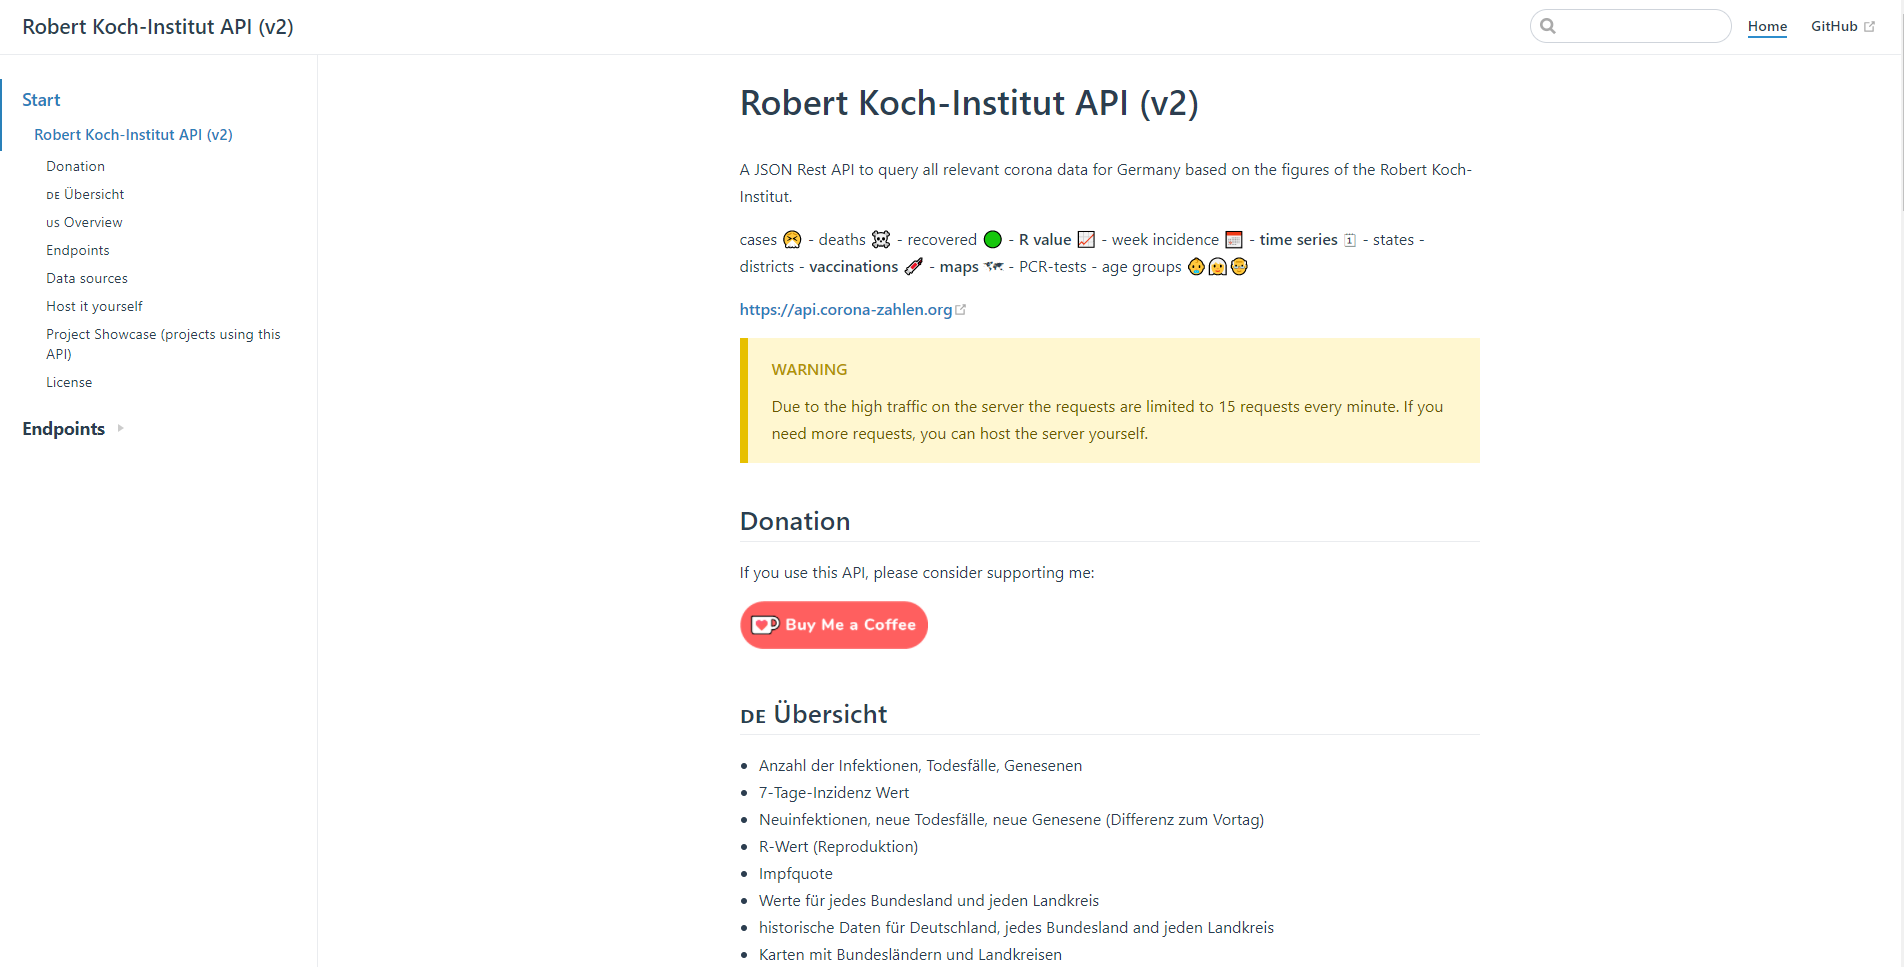
\includegraphics[scale=0.4]{rkiapiOverview.png}
	\captionsetup{justification=centering}
	\caption{RKI Corona API Startseite}
	\label{pic:rkiapiOverview}
\end{figure}

\section{Corona Maßnahmen}
Für die Daten der gültigen Maßnahmen und Verordnungen wird direkt auf die offiziellen Websites der Bundesregierung bzw. der jeweiligen Landesregierung zugegriffen. Wir haben uns bewusst dagegen entschieden mögliche Dritt-Anbieter wie Nachrichtenportale zu integrieren um die Informationen ungefiltert zu erhalten, was auch Nachteile nach sich zog da die jeweiligen Regierungsportale es teilweise deutlich schwerer gemacht haben. Daraus resultieren 16 Webseiten die als Datenquellen hergenommen werden, hier eine Übersicht:

\begin{itemize}
\itemsep-1em
\item \url{https://www.stmgp.bayern.de/coronavirus/}
\item \url{https://www.niedersachsen.de/Coronavirus/vorschriften-der-landesregierung-185856.html}
\item \url{https://www.hamburg.de/verordnung/}
\item \url{https://www.inneres.bremen.de/corona-die-haeufigsten-fragen-und-antworten-23460}
\item \url{https://kkm.brandenburg.de/kkm/de/}
\item \url{https://www.berlin.de/corona/massnahmen/verordnung/}
\item \url{https://corona.rlp.de/de/aktuelles/corona-regeln-im-ueberblick/}
\item \url{https://www.saarland.de/DE/portale/corona/service/downloads/_documents/corona-verfuegungen/dld_2021-08-25-aenderung-vom-21-08-18.html}
\item \url{https://www.schleswig-holstein.de/DE/Schwerpunkte/Coronavirus/Erlasse/2021/210820_LF_corona-bekaempfungsvo.html}
\item \url{https://www.baden-wuerttemberg.de/de/service/aktuelle-infos-zu-corona/aktuelle-corona-verordnung-des-landes-baden-wuerttemberg/}
\item \url{https://www.coronavirus.sachsen.de/amtliche-bekanntmachungen.html}
\item \url{https://coronavirus.sachsen-anhalt.de/amtliche-informationen/}
\item \url{https://www.hessen.de/fuer-buerger/corona-hessen/verordnungen-und-allgemeinverfuegungen}
\item \url{https://www.tmasgff.de/covid-19/verordnung}
\item \url{https://www.land.nrw/de/media/galerie/corona-fakten-1}
\item \url{https://www.regierung-mv.de/corona/Verordnungen-und-Dokumente/}
\end{itemize}

Im laufe der Analyse der Websites stellte sich heraus das es drei Fälle zu Beleuchten gab. Zum einen wurde oft auf den Websites mehr schlecht als recht über die aktuellen Corona-Maßnahmen informiert und nur auf das aktuell gültige Rechtsdokument wie eine Corona-Verordnung verwiesen welches meistens als PDF-Datei publik gemacht wurde:
\begin{figure}[H]
\caption{Hessische Landesseite (Verordnung als PDF verlinkt)}
\label{websiteHessen}
\centering

\includegraphics[scale=0.9]{pictures/hessenOverview.png}
\end{figure}

Seltener wurde die gültige Verordnung oder zusammengefasste Informationen als reiner Text in den HTML-Code integriert:

\begin{figure}[H]
\caption{Berliner Landesseite (Verordnung im HTML Code)}
\label{websiteBerlin}
\centering
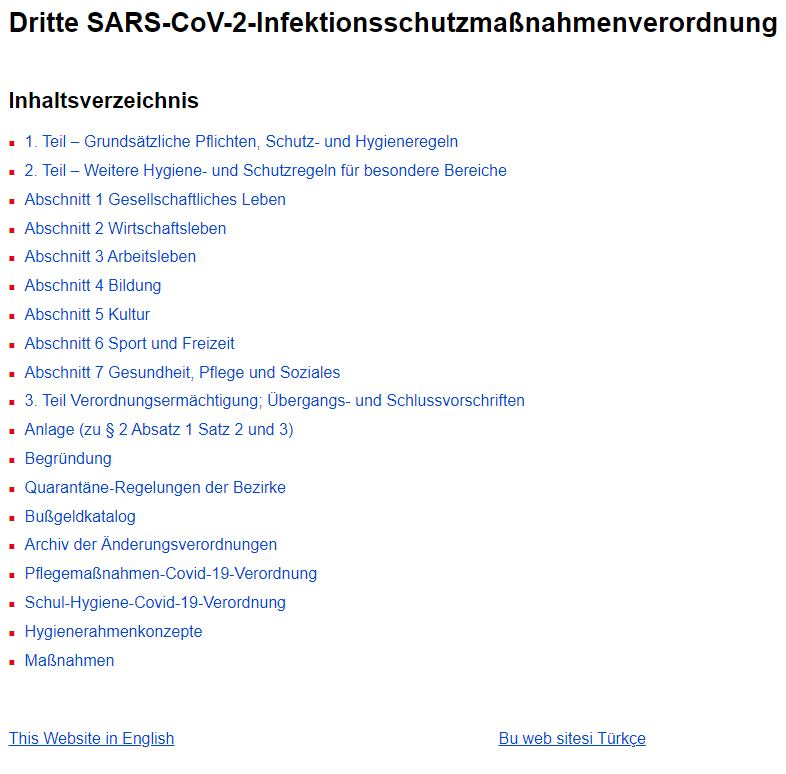
\includegraphics[scale=0.8]{pictures/berlinOverview.png}
\end{figure}

Und letzteres wurden zusammengefasste Informationen als Überblick in einer Bildergalerie präsentiert:

\begin{figure}[H]
\caption{Nordrhein-Westfalens Landesseite (Informationen als Bilder Galerie)}
\label{websiteNRW}
\centering

\includegraphics[scale=0.8]{pictures/nrwOverview.png}
\end{figure}

\section{Wetterdaten}
Die Wetterdaten sind grunds\"atzlich die einfachste Datenquelle. Hier gibt es mehrere verschiedene APIs die Wetterdaten zur Verfügung stellen, die Schwierigkeit ist nur eine API zu finden die diese Informationen ohne Kosten freigeben.
Ausgew\"ahlt wurde hier endg\"ultig \textit{https://openweathermap.org/api}. Hier k\"onnen aktuelle Wetterdaten umsonst heruntergeladen werden. Eingeschr\"ankt wird hier bei historischen Daten, was allerdings f\"ur das Konzept irrelevant ist da die Daten immer tagesaktuell abgespeichert werden sollen. \newline
Die API wird dann pro Stadt abgefragt und nach dem Ablagekonzept abgelegt bzw. indiziert. Zu beachten ist allerdings noch das nur eine beschr\"ankte Anzahl an Anfragen pro Minute durchgef\"uhrt werden k\"onnen. Dies wurde Software technisch Umgang oder besser gesagt ber\"ucksichtigt.

\chapter{Problemstellung}
\section{Corona Maßnahmen}
Bei den bereits genannten Datenquellen ergab sich die Problematik dass die Informationen in unterschiedlichen Formaten vorhanden sind. Die Informationen waren in Bildern als JPEG- und PNG-Dateien sowie PDF-Dateien enthalten und als reiner Text in den HTML-Code eingebettet. Um an die Rohdaten zu kommen wäre es an dieser Stelle ein leichtes diese Dateien nun einfach herunterzuladen und im HDFS abzulegen, da wir aber auch Metadaten für spätere Analysen speichern möchten hatten wir das Problem das wir aus den Bildern und PDF Dateien die Informationen extrahieren mussten. Um die Bilder zu Text zu wandeln entschieden wir uns für die Open Source OCR Engine Tesseract und um den Text aus den PDFs während der Laufzeit zu erhalten wurde auf das Python-Package pdfminer.six gesetzt.

\subsection{Tesseract}
Tesseract wurde ursprünglich bei Hewlett-Packard entwickelt und 2005 als Open Source veröffentlicht wo es seit 2006 von Google betreut wird.
Seit Version 4 wurde die Engine auf ein künstliches Neuronales Netz aufgebaut. Grundsätzlich wird die Software von der Kommandozeile aus gesteuert. Um es aus unserem Python-Skript ansprechbar zu machen wird dazu noch das pytesseract-Package für Python benötigt.

\subsubsection{Bildumwandlung}\label{sec:sub:sub:bild}
Während der Entwicklung und Verwendung von Tesseract ist aufgefallen das die Engine mit einigen bunten Bildern, die die Landesregierungen veröffentlicht haben Probleme hat. Vor allem wenn der Text farbig auf farbigen Hintergrund ist. Um dieses Problem schnell und trotzdem effizient zu lösen haben wir uns entschieden die Bilder vor der Textanalyse in schwarz und weiß umzuwandeln. Verschiedene Tests und die bisherige Erfahrung haben gezeigt dass das zwar keine perfekte aber durchaus eine solide Lösung ist.

\chapter{Funktion und Implementierung}

Für unsere vier primären Datenquellen RKI Daten, Maßnahmen der Regierung, Nachrichtenartikel und Wetterdaten haben wir uns Entschieden jeweils ein eigenes Programm ('Scraper') mit Python zu implementieren die hier nun einzeln erläutert werden. \newline

\section{Scheduling}
Jeder der Scraper wird, wie in Sektion \ref{ooziecron} bereits erwähnt, mit Cron gestartet. Als Zeitintervall wurde eine Stunde gewählt (siehe \ref{cron}). \newline

\begin{lstlisting}[caption=Cron-einstellungen,label=cron,language=bash]
#M   S     T M W   Befehl
#-----------------------------------------------------------------
0 * * * *   /home/hadoop/ArticleScraper/ubuntu_venv/bin/python3 /home/hadoop/ArticleScraper/main.py
0 * * * *   /home/hadoop/RKILoader/venv/bin/python3 /home/hadoop/ArticleScraper/main.py
0 * * * *   /home/hadoop/weatherdownloader/venv/bin/python3 /home/hadoop/ArticleScraper/main.py
0 * * * *   /home/hadoop/ArticleScraper/ubuntu_venv/bin/python3 /home/hadoop/ArticleScraper/main.py
#-----------------------------------------------------------------
\end{lstlisting}

\pagebreak

\section{Maßnahmen}

\subsection{Konfigurationen}

\subsubsection{Programm Konfiguration}
Bei der Entwicklung wurde auf hohe Konfigurierbarkeit geachtet da schon während des Prozesses festgestellt wurde das jederzeit Änderungen an den ausgewählten Websiten passieren können und deshalb das Programm sehr flexibel sein sollte. Hierfür wurde eine Config.py-Datei angelegt in denen alle wichtigen Informationen wie z.B. URLs von ElasticSearch und HDFS etc.

\begin{lstlisting}[caption=Config für das Programm]
# -------------------------------hdfs--------------------------------
HDFS_BASE_URL = '127.0.0.1'
HDFS_PORT = '50070'
HDFS_USER = 'hadoop'
HDFS_MEASURES_BASE_PATH = '/datakraken/measures/'
# -------------------------------TESSERACT---------------------------
TESSERACT_PATH = "E:/Programme/Tesseract/tesseract"
# -------------------------------logging-----------------------------
loggerName = "restrictionLogger"
logFileName = 'RestrictionScraper.log'
# -------------------------------ElasticSearch-----------------------
es_url = '127.0.0.1'
es_port = '9200'
indexName = "restrictions"
...
\end{lstlisting}

\pagebreak

\subsubsection{Datenquellen Konfiguration}
Da fast auschließlich nur spezielle Elemente der Websiten wie die \textless a\textgreater -Tags der PDFS oder  \textless img\textgreater -Tags der Bilder selektiert werden mussten wurde auf ein Key/Value-Schema zurückgegriffen. Der Key spezifierte ob der Code auf eine spezielle Element-ID oder ein Klassenname durchsucht wird, falls das aber nicht möglich war wurde auf den eindeutigen CSS Selector des Elements zurückgegriffen.

\begin{figure}[H]
\caption{HTML-Element der Hessischen Landesseite}
\label{htmlHessen}
\centering
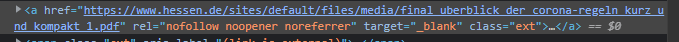
\includegraphics[scale=1.0]{pictures/hessenHTMLexample.png}
\end{figure}

Wie man in \cref{htmlHessen} sehen kann ist das \textless a\textgreater -Tag nicht über eine Id oder ähnliches eindeutig selektierbar deswegen wird ein CSS Selector gebildet, den man sich zudem auch über die Entwicklertools generieren kann. In diesem Beispiel:
\begin{lstlisting}[caption=CSS Selector]
#node-listenseite-100174 > div.content.clearfix > div.view.view-registerblock.view-id-registerblock.view-display-id-block.view-dom-id-eabeac53f51705a80d47815e52e2470f.hzd_registerpage-processed > div > div.views-row.views-row-1.views-row-first.views-row-odd > div.views-field.views-field-nothing-2.registerpage-content-right.he_content_body > div > a
\end{lstlisting}

Zu jedem Bundesland wurde eine Konfiguration in ElasticSearch gespeichert die am Anfang des Programms geladen wird und dementsprechend dann die Daten lädt.

\begin{lstlisting}[caption=Config von Bayern, language=json]
{
	"state" 	: "Bayern",
	"url"	: "https://www.stmgp.bayern.de/coronavirus/",
	"Target": "class_",
	"Value"	: "vc_single_image-img attachment-full"
}
\end{lstlisting}

\subsection{Programmablauf}

\begin{figure}[H]
\caption{Aktivitätsdiagramm des Scrapers}
\label{activityRestriction}
\centering
\includegraphics[scale=0.5]{pictures/aktivitätsdiagramm_restrictionscraper.png}
\end{figure}

\subsubsection{Rohdaten Extrahierung}\label{sec:sub:sub:rohdaten}

Wie im Aktivitätsdiagramm \cref{activityRestriction} zu sehen ist, werden am Anfang alle Datenquellenkonfigurationen aus ElasticSearch geladen und der Scraping Prozess für jede Quelle gestartet. Hierbei wird auf die in der Config angegebene URL zugegriffen und die jeweiligen Elemente die durch Target/Value spezifiert sind heruntergeladen. Dazu wird auf die Python-Bibliothek BeautifulSoup zurückgegriffen die zum parsen von XML- und HTML-Dokumenten dient.

\begin{lstlisting}[caption=Parsen und filtern der Website, language=Python]
	page = requests.get(self.baseUrl)
       soup = BeautifulSoup(page.content, 'lxml')
        if self.target == 'CSSselector':
            elements = soup.select(self.val)

        else:
            kwargs = {
                    self.target: self.val
                }
            elements = soup.find_all(**kwargs)
\end{lstlisting}

Nachdem die Elemente extrahiert wurden wird je nach Fall weiter verfahren. Wenn es eine Bild-URL ist wird das Bild herunter geladen. Um mit Tesseract eine höhere Genauigkeit zu erzielen wie in \cref{sec:sub:sub:bild} beschrieben, werden die Bilder zu schwarz-weiß konvertiert. Im HDFS werden beide Varianten der Bilder abgespeichert und das konvertierte Bild wird Tesseract zur Textumwandlung übergeben.
% TODO installation tesseract etc erklären vll bei setup (sprachpakete etc)

\begin{lstlisting}[caption=Schwarz-weiß Konvertierung, language=Python]
	imgBytes = requests.get(cleanedUrl).content
	image = Image.open(io.BytesIO(imgBytes))
	imgBW = image.convert("1", dither=Image.NONE)
	self.hdfs_client.save_as_file(self.directory, fileNameBW, imgBWbytes)
	self.hdfs_client.save_as_file(self.directory, fileName, imgBytes)

	data = pytesseract.image_to_string(imgBW, lang='deu')
\end{lstlisting}

Im Falle eines verlinkten PDF-Dokuments wird dieses herunter geladen und der Text mit der Bibliothek pdfminer.six extrahiert.

\begin{lstlisting}[caption=PDF Text Extraktion, language=Python]
	fileBytes = requests.get(url).content
	self.hdfs_client.save_as_file(self.directory, fileName, fileBytes)
	data = pdfminer.high_level.extract_text(io.BytesIO(fileBytes), codec="utf-8")
\end{lstlisting}

Der letzte Fall bedeutet das die Informationen direkt im HTML-Code als Text integriert sind. Hierbei laden wir einfach die komplette Seite und extrahieren den Text hieraus.

\begin{lstlisting}[caption=Website speichern, language=Python]
	response = urllib.request.urlopen(self.baseUrl)
      webContent = response.read()
	self.hdfs_client.save_as_file(self.directory, str(time.time())+
		_+DEFAULT_HTML_FILENAME, webContent)
	data = elem.text.strip()
\end{lstlisting}

\subsubsection{Metadaten Extrahierung}

Nachdem in \cref{sec:sub:sub:rohdaten} die Rohdaten gespeichert wurden und der Text daraus extrahiert wurde ging es darum sinnvolle Metadaten zu filtern. Eine sinnvolle und robuste Verarbeitung zu finden war eine große Herausforderung - um daraus nicht eine neue Projektarbeit vom Zaun zu brechen wurde auf simple Methoden wie String vergleiche und verstärkt auf reguläre Ausdrücke gesetzt. Zu Beginn der Entwicklung war der Inzidenzwert die maßgebliche Metrik zur Bewertung der Situation im Gegensatz zur Krankenhausbelegung derzeit. Deswegen wurde unter anderen der Text darauf analysiert ob die Maßnahme Inzidenzbasierend ist und wenn ja, welche Inzidenzschranken vorhanden sind. Des weiteren wird ein Gültigkeitsdatum gesucht und der Text auf diverse Tags wie Maskenpflicht, Kontaktbeschränkungen etc. untersucht um die Maßnahme etwas eingrenzen zu können. Hierfür wurden diverse reguläre Ausdrücke verwendet z.B.

\begin{lstlisting}[caption=Regex für Inzidenzschranken, language=Python]
INCIDENCE_REGEX =
	r"(((?<=Inzidenzstufe)|(?<=Inzidenzwert)
	|(?<=Inzidenz)|(?<=Schwellenwert))).{0,20}(\d{2,3})"
\end{lstlisting}

Am Ende werden die json-Objekte mit folgendem Format an ElasticSearch gesendet:

\begin{lstlisting}[caption=Metadaten-Objekt, language=json]
{
	"validFrom": "19-08-2021",
	"incidenceBased": false,
	"federateState": "Hessen",
	"creationDate": "07-09-2021",
	"incidenceRanges": null,
	"tags": [
		"Maskenpflicht",
		"Veranstaltungen",
		"Kultur",
		"Schule",
		"Sport"
	]
}
\end{lstlisting}

Um zu verhindern das die selben Maßnahmen immer wieder neu extrahiert werden wird jedes mal beim indexieren in ElasticSearch eine unique ID mitgeben die sich aus dem Bundesland plus dem Gültigkeitsdatum der Maßnahme bildet. Vor jedem Einfügen wird zuerst geprüft ob dazu schon ein Datensatz existiert und nur wenn nicht dann wird die Aktion vollzogen.

\subsection{Persistierung}

\subsubsection{HDFS Wrapper}

Um die Daten ohne Probleme ins HDFS einfügen zu können wurde auf die 'pywebHDFS' Bibliothek in Python zurückgegriffen. Diese bildet für uns die Schnittstelle zwischen unserem Code und dem Dateiablagesystem. Um das ganze isoliert nutzen zu können wurde eine HDFS Wrapper Klasse geschrieben die, die Funktionalität von pywebhdfs beinhaltet.

\subsubsection{ElasticSearch Wrapper}

Genauso wurde für die ElasticSearch Anbindung auf deren veröffentlichte Python-Bibliothek ElasticSearchClient aufgebaut. Auch hier wurde wieder eine Wrapper Klasse geschrieben zur Kapselung.
\pagebreak


\section{Artikel}


\subsection{Programmaufbau und Ablauf}

\begin{figure}[h!]
\caption{Klassendiagram(vereinfacht)}
\label{articlescraperclassdiag}
\centering
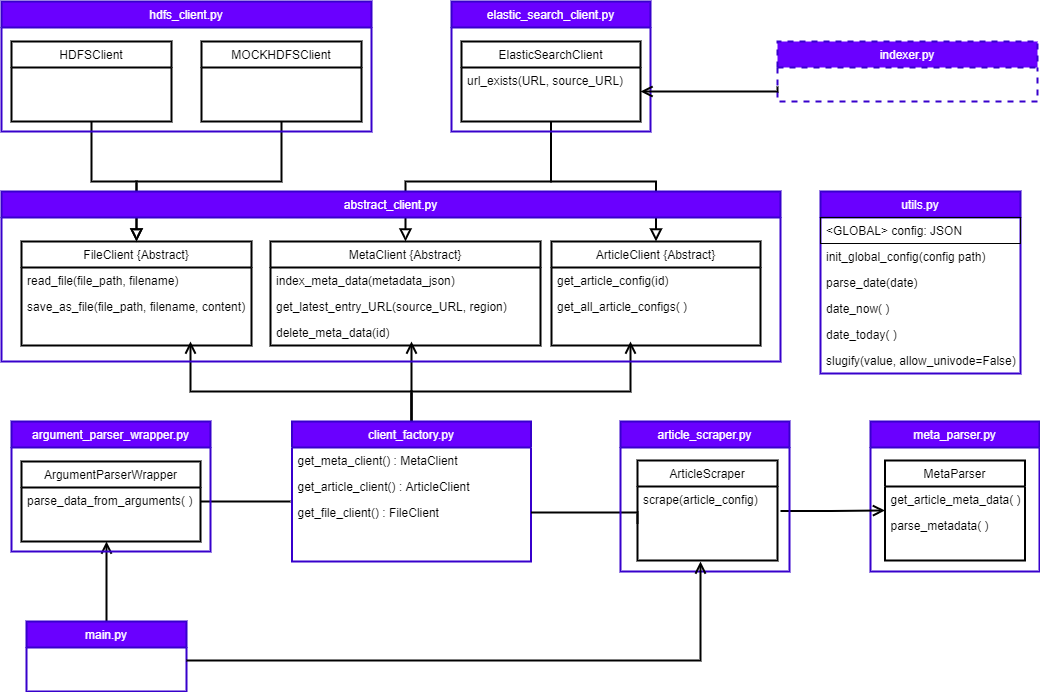
\includegraphics[scale=0.4]{article_scraper_class_diagram.png}
\end{figure}
Der Übersichtlichkeit halber wurden im oberen Diagram \ref{articlescraperclassdiag} 'private' Funktionen sowie lose Kuppelungen mit dem Modul 'utils.py' weggelassen. Das Modul 'indexer.py' nimmt eine Sonderrolle ein, da es einzig dazu dient article\_configs aus JSON-Dateien in Elasticsearch zu indizieren, sonst aber nichts mit dem eigentlichen Programm zu tun hat. Das Programm kann logisch in die Module abstract\_client.py, client\_factory.py, hdfs\_client.py und elastic\_search\_client.py welche der Persistierung der Daten dienen und argument\_parser\_wraper.py, article\_scraper.py und meta\_parser.py welche das Extrahieren und Verarbeiten der Daten übernehmen unterteilt werden. Diese Unterteilung dient der Austauschbarkeit von Komponenten und der Trennung von Fachdomäne und Infrastruktur wie im Domain-Driven-Design üblich.
\pagebreak


\begin{figure}[h!]
\caption{Swimlane diagram(vereinfacht)}
\label{articlescraperswimlanediag}
\centering
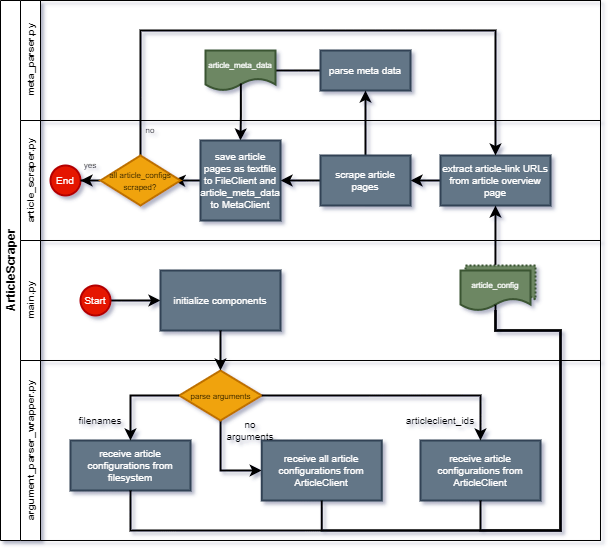
\includegraphics[scale=0.6]{article_scraper_swimlane_diagram.png}
\end{figure}
Im oberen Diagram \ref{articlescraperswimlanediag} wurden die einzelnen Clients aus Gründen der Übersichtlichkeit nur in Textform erwähnt.
\pagebreak


\subsection{Konfigurierbarkeit}
Um mit dem Scraper später von beliebigen Quellen scrapen zu können wurde das gesamte System so konfigurierbar wie möglich gemacht. Hierfür waren 2 Arten von Konfigurationsdateien notwendig, eine für das gesamte System und eine für jede Quelle von der mit dem Programm gescraped werden soll. Alle Konfigurationen wurden im JSON-Format abgespeichert, im folgenden das Format der JSON-Dateien(Listing \ref{config} und Listing \ref{articleconfig}), auf deren Anteile wir später weiter eingehen.


\subsubsection{Allgemeine Konfiguration}
Die allgemeine Konfiguration config.json wird bei Start in eine globale Variable eingelesen auf die von überall aus zugegriffen werden kann. Werte aus dieser Datei können sich grob in Daten zur Initialisierung der Clients und des Loggers, sowie Zeitformate und Einstellungen für den Scraper einteilen.
\begin{lstlisting}[caption=config.json,label=config,language=json]
{
"ELASTICSEARCH_URL" : "192.168.0.115",
"ELASTICSEARCH_PORT" : "9200",
"HDFS_URL" : "192.168.0.115",
"HDFS_PORT" : "9870",
"HDFS_USER" : "hadoop",
"RECENT_ARTICLE_COUNT" : "100",
"MAX_TRY" : "3",
"STANDARD_DATETIME_FORMAT" : "%Y-%m-%dT%H:%M:%S.%fZ",
"STANDARD_DATE_FORMAT" :"%Y-%m-%d",
"STANDARD_LOG_FORMAT" : "[%(levelname)s][%(asctime)s]: %(message)s",
"STANDARD_LOG_DATE_FORMAT" : "%Y-%m-%d %H:%M:%S",
"STANDARD_LOG_FILENAME" : "articlescraper.log",
"WEBDRIVER_DIR" : "drivers",
"WEBDRIVER_FILE" : "chromedriver",
"CLIENTS" : {
    "META_CLIENT" : "elastic",
    "ARTICLE_CLIENT" : "elastic",
    "FILE_CLIENT" : "hdfs"
}
}
\end{lstlisting}


\subsubsection{Artikel Konfiguration}
Die Artikelkonfiguration ( im weiteren nur article\_config) kann entweder aus dem gleichnamigen Datenbank-Index( Hier von  Elasticsearch ) geladen oder aus einer JSON-Datei gelesen werden. Hierfür wird argparse benutzt, mit welchem sich Commandlineargumente einstellen und parsen lassen. Für den ArticleScraper sind die vorhandenen Optionen:
\begin{itemize}
\item --articleclient \textless id\textgreater: Die unter dem Index "article\_config" hinterlegte Konfiguration mit entsprechender \textless id\textgreater wird gescraped
\item --file \textless filename\textgreater: Die unter dem \textless filename\textgreater gefundene Datei wird gescraped
\item keine Argumente: Alle unter dem Index "article\_config" hinterlegten Konfigurationen werden gescraped
\end{itemize}
Die entsprechenden Konfigurationen werden dann als Liste dem Scraper zurückgegeben und weiter verarbeitet.
\begin{lstlisting}[caption=article\_config am Beispiel Niedersachsen,label=articleconfig,language=json]
{
    "region": "niedersachsen",
    "site_name": "kreiszeitung",
    "base_url": "https://www.kreiszeitung.de/",
    "path_url": "suche/?tt=1&tx=&sb=&td=&fd=&qr=corona",
    "html_tag": "div",
    "html_class": "id-LinkOverlay",
    "url_conditions" : [
        {
        "condition_string": "/niedersachsen",
        "include_condition": true}
        	],
    "title": {
        "source": "TAG",
        "tag": "meta",
        "attribute" : "property",
        "attribute_value": "og:title"
    },
    "date": {
        "source": "TAG",
        "tag": "meta",
        "attribute" : "property",
        "attribute_value": "article:published_time"
    },
    "author": {
        "source": "JSON_LD",
        "tag": "author",
        "attribute" : null,
        "attribute_value": null,
        "default": null
    },
    "description": {
        "source": "TAG",
        "tag": "meta",
        "attribute" : "property",
        "attribute_value": "og:description",
        "default": null
    },
    "type": {
        "source": "DEFAULT",
        "tag": null,
        "attribute" : null,
        "attribute_value": null,
        "default": "anschauungszweck erfuellt"
    },
    "keywords": {
        "source": "NOEXIST",
        "tag": null,
        "attribute" : null,
        "attribute_value": null,
        "default": null
    }
}
\end{lstlisting}
\pagebreak


\subsection{Erhalten von Artikellinks}
\begin{figure}[h]
\caption{Übersicht der Suchergebnisse Kreiszeitung}
\label{articlelist}
\centering
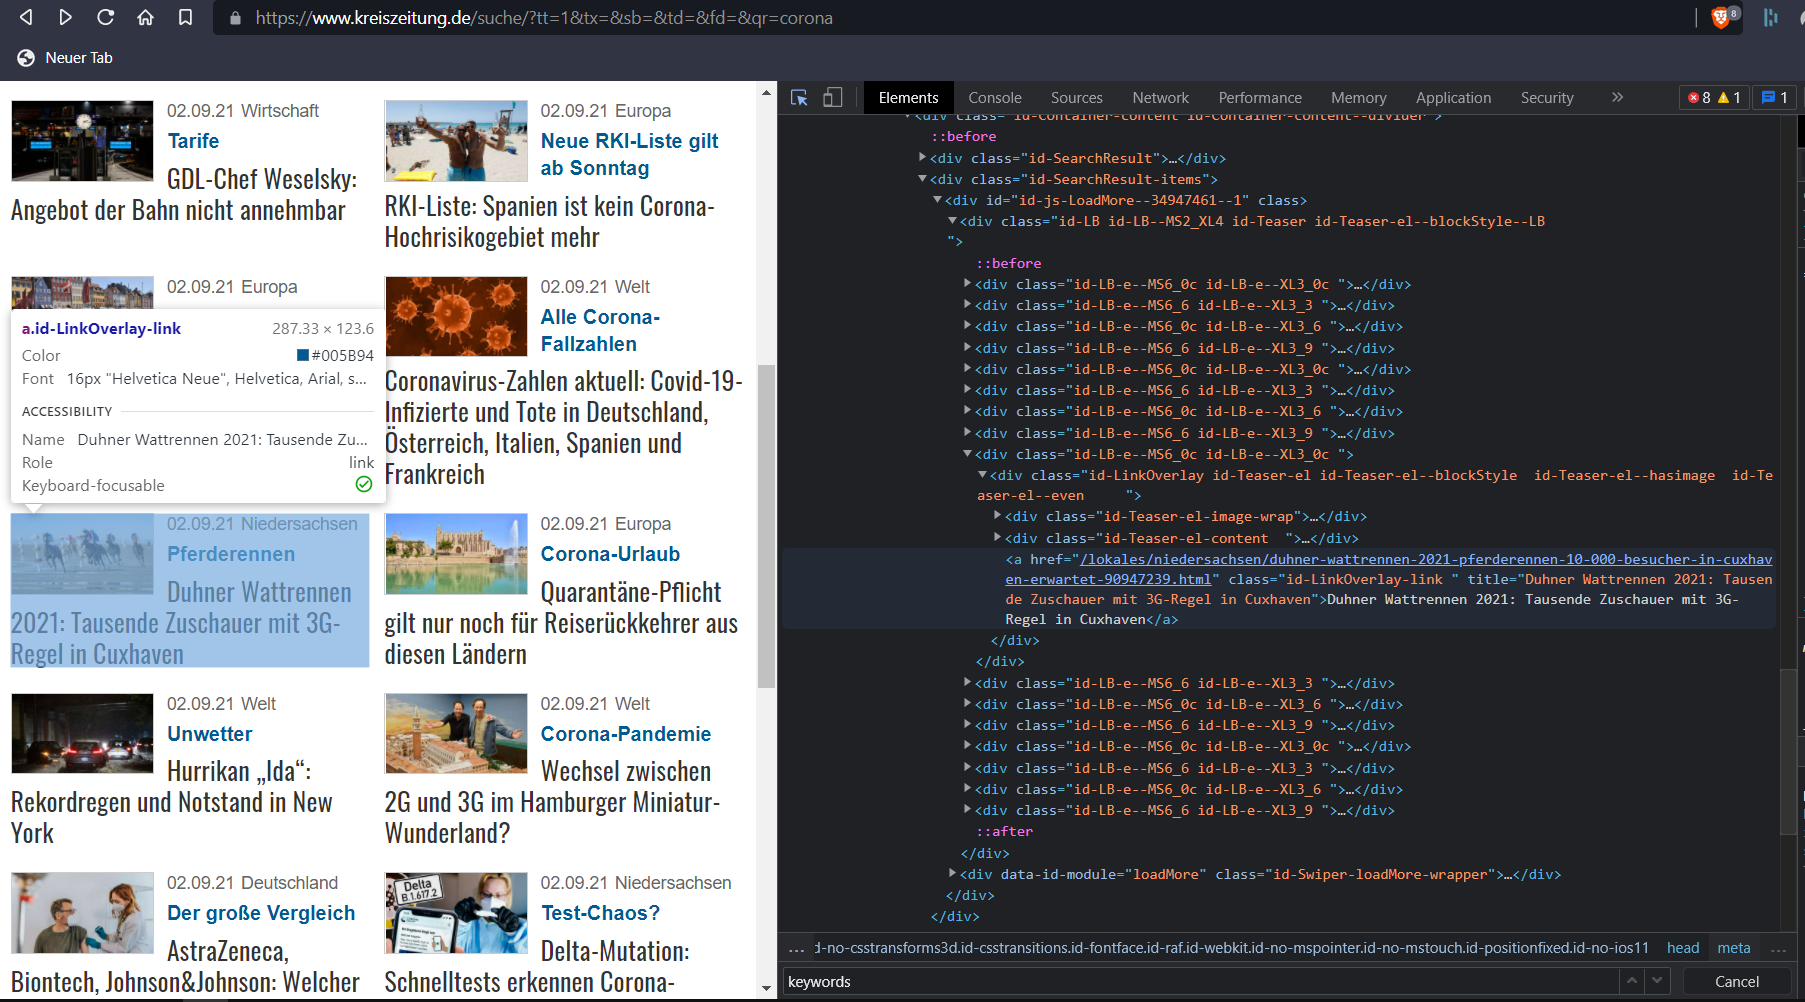
\includegraphics[scale=0.4]{articles_list.png}
\end{figure}

Um nicht jedes mal für jeden einzelnen Artikel eine eigene Konfiguration erstellen bzw. einen Scrapevorgang starten zu müssen wird sich zu nutze gemacht, dass Artikelverlinkungen auf Artikelübersichtsseiten, wie in Figure \ref {articlelist} zu sehen, in gleichartige HTML-Tags geschrieben werden. 

\begin{lstlisting}[caption=article\_config für Übersichtsseite,label=articleconfigoverview,language=json]
    "base_url": "https://www.kreiszeitung.de/",
    "path_url": "suche/?tt=1&tx=&sb=&td=&fd=&qr=corona",
    "html_tag": "div",
    "html_class": "id-LinkOverlay",
    "url_conditions" : [
        {
        "condition_string": "/niedersachsen",
        "include_condition": true}
        	],
\end{lstlisting}

Es muss in der article\_config also nur der Link zu dieser Übersichtsseite (bestehend aus base\_url und path\_url), sowie das HTML-Tag(html\_tag) und die HTML-Klasse(html\_class) angegeben werden. Im Fall des Beispiels in listing \ref{articleconfigoverview} wurden die Artikel der Kreiszeitung bereits über eine suche, wie unter path\_url zu sehen weiter auf unser Themengebiet eingeschränkt. 
\pagebreak

Die URLs der einzelnen Artikel werden dann in 3 Schritten extrahiert. \newline
Im ersten Schritt werden alle passenden Tags herausgefiltert. \newline
Im zweiten Schritt wird die URL aus jedem Tag bzw. seinen descendants extrahiert. \newline
Im dritten und letzten Schritt wird diese Liste aus Links gefiltert. Es wird nun verhindert, dass unerwünschte Artikel wie z.B. Werbung, Newsticker und Ähnliches gespeichert werden. Hierzu lassen sich über 'url\_conditions' bei 'url\_string' Zeichenketten angeben, welche in der URL des Artikels (nicht) vorkommen sollen, steuerbar über setzen von 'include\_condition' auf true/false. Dabei lässt sich durch die Elemente der Liste eine 'AND'-Beziehung darstellen, über trennen von Zeichenketten mittels '\textbar' innerhalb eines 'condition\_string' eine 'OR'-Beziehung. In diesem Beispiel werden Artikellinks nach dem kriterium gefiltert, ob sie '/niedersachsen' enthalten, den Pfad der Website, unter welchem alle Niedersachsen betreffenden Artikel zu finden sind. \newline
Weiter wird die Liste nach URLs gefiltert, welche bereits in einem vorherigen Scrapevorgang verarbeitet wurden. Hierzu wird eine Anzahl der letzten gespeicherten Artikel-Metadaten geladen und mit der Linkliste abgeglichen. Um den Scraper so generisch wie möglich zu halten wurde bewusst darauf verzichtet an dieser Stelle die Liste nur mit dem aktuellsten gespeicherten Artikel-Metadatensatz abzugleichen und dann abzubrechen, da es bei manchen Webseiten zu Fehlern aufgrund von abweichender Sortierung kam.
\pagebreak

\subsection{Sammeln von Metadaten}
Es werden zu jedem Artikel Metadaten gespeichert um später einmal schnell Artikel nach bestimmten Kriterien suchen und filtern zu können. Hierzu wird in der article\_config, wie in Listing \ref{articleconfig} zu sehen, zu jedem der ausgewählten Attribute spezifiziert, wo diese im HTML-Dokument der Seite zu finden sind bzw. wie sie zu definieren sind. Es stehen 4 Optionen für Quellen zur Verfügung: 
\begin{itemize}
\item \textbf{TAG} \newline
\begin{figure}[h!]
\caption{Metadaten in HTML-Dokument}
\label{articlemeta}
\centering
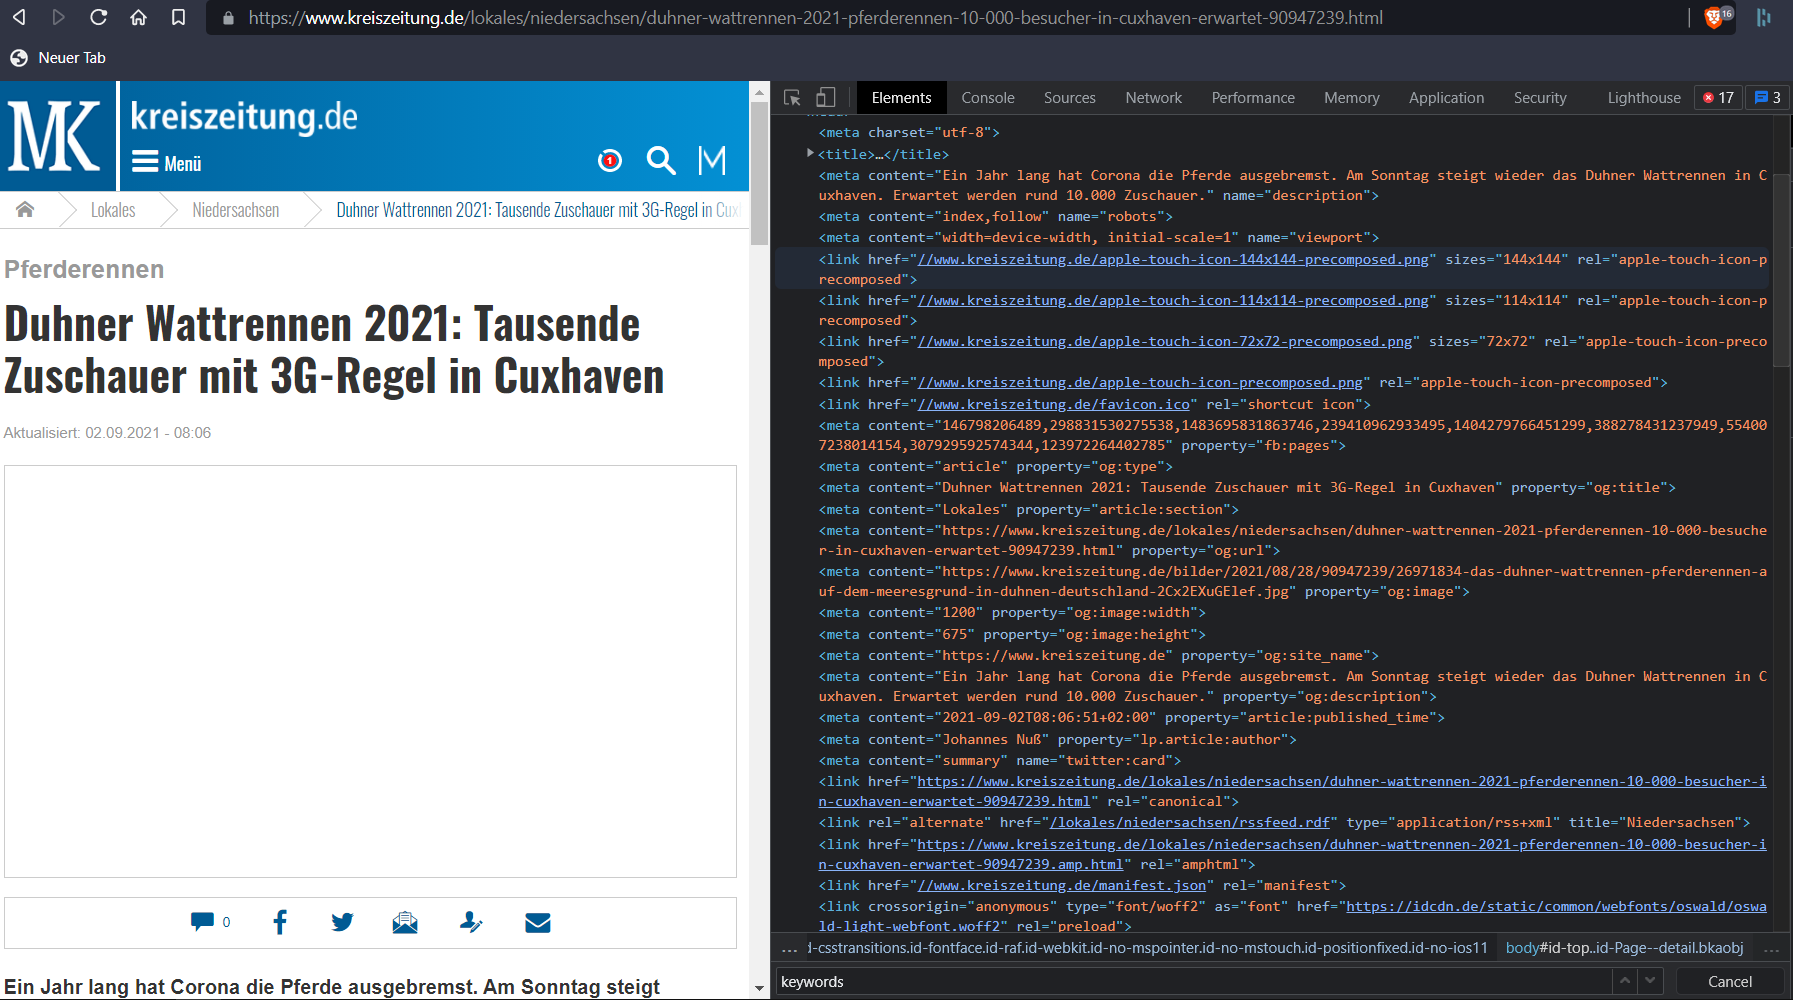
\includegraphics[scale=0.4]{articles_meta.png}
\end{figure} \newline
Die gesuchte Information kann in einem Tag gefunden werden. Dies beinhaltet alle 'normalen' Tags, es können Informationen aus dem Text des Tags oder aus dem 'content' extrahiert werden, wobei Text vorrang hat. über 'tag', 'attribute' und 'attribute\_value' können die benötigten Tags, wie in Listing \ref{articleconfig} auf Basis von Abbildung \ref{articlemeta} zu sehen, weiter spezifiziert werden.


\item \textbf{DEFAULT} \newline
Die gesuchte Information soll einen Defaultwert annehmen. Dieser wird in der article\_config über das Attribut 'default' bestimmt (siehe Listing \ref{articleconfig}). Dies gilt nicht für 'title', der für die Benennung der zu speichernden Datei benötigt wird. Für 'date' wird der aktuelle Zeitpunkt genommen.

\pagebreak

\item \textbf{JSON\_LD}\newline
\begin{figure}[h!]
\caption{Metadaten in HTML-Dokument}
\label{articlejson}
\centering
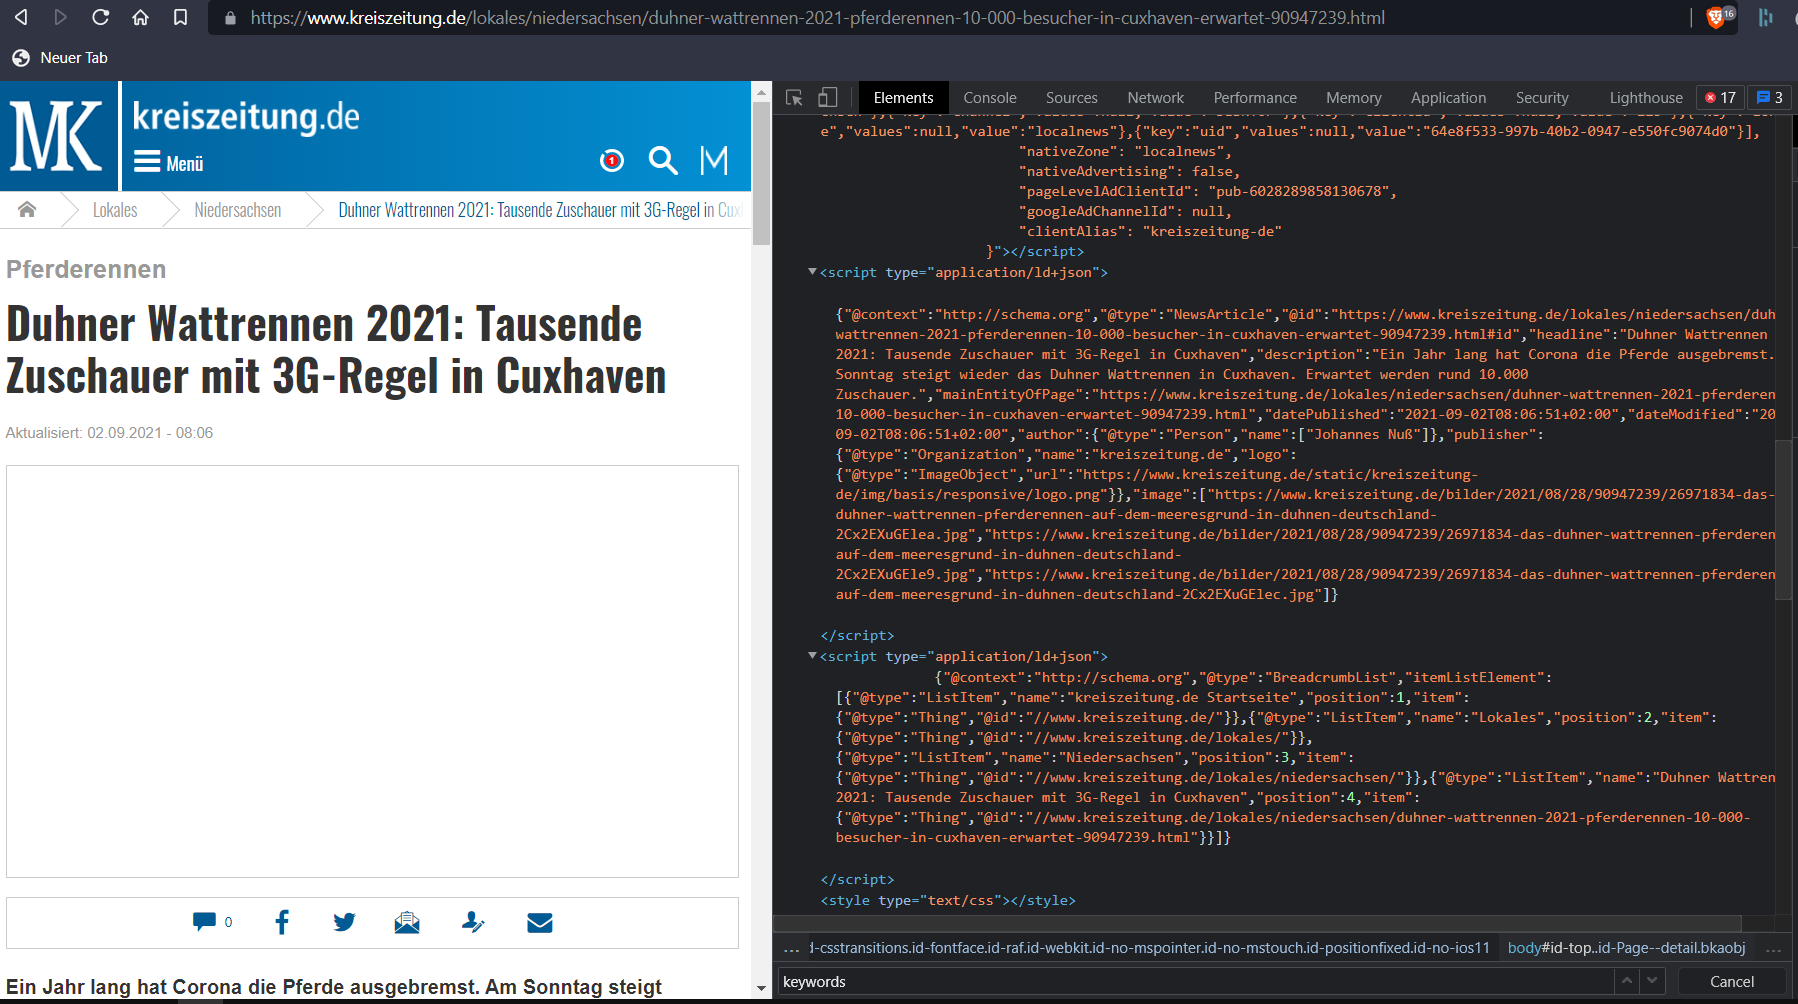
\includegraphics[scale=0.4]{articles_ld_json.png}
\end{figure} \newline
 Die gesuchte Information kann in einem eingebetteten JSON im 'script'-Tag vom Typ 'application/ld+json', wie in Abbildung \ref{articlejson} zu sehen, gefunden werden. Über die Attribute 'attribute' und 'attribute\_value', der article\_config, können einzelne Tags ausgewählt werden. Für die Auswahl des Wertes wird das 'tag' Attribut der article\_config als Key genutzt. Dabei ist es möglich auch verschachtelte oder Listenelemente zu extrahieren. Sollte der gefundene JSON-Key auch wieder ein Dictionary sein wird der Value des Key 'name' extrahiert (zu sehen in Abbildung \ref{articlejson} und Listing \ref{articleconfig}). 

\item \textbf{NOEXIST} \newline
Die Information steht nicht zur Verfügung oder soll nicht gespeichert werden. Es wird stattdessen ein Bindestrich als Freizeichen gespeichert.
\end{itemize}

\pagebreak

Anhand dieser Festlegungen wird für jedes Attribut eine passende Strategie angewendet. Die so gewonnenen Informationen werden in das JSON-Dokument 'article\_meta\_data' geschrieben.
\begin{lstlisting}[caption=article\_meta\_data Dokument vor seiner Befüllung mit Daten,label=articlemetadata,language=json]
{ 	 
	"title" : None, 
	"description" : None, 
	"url": URL, 
	"source_url" : article_config["base_url"] + article_config["path_url"],  
	"type" : None, 
	"date" : None, 
	"index_time" : utils.date_now(),
	"region" : article_config["region"], 
	"site_name" : article_config["site_name"], 
	"author" : None, 
	"keywords" : None,
	"filename" : "placeholder_to_prevent_iteration",
	"filepath" : "placeholder_to_prevent_iteration"
}
\end{lstlisting}
In Listing \ref{articlemetadata} sind neben denen aus dem HTML-Dokument noch weitere Attribute zu sehen. Bei 'source\_url', 'region' und 'site\_name' handelt es sich um Informationen welche aus der 'article\_config' übernommen werden, da deren benennung dem Nutzer überlassen werden soll bzw. im Falle der 'source\_url' nicht mehr zugänglich ist. 'index\_time' hält den Zeitpunkt der Erstellung des Dokuments fest (Nicht den der Indizierung) und 'filename' und 'filepath' dienen zum abspeichern und wiederfinden der Datei und werden erst u.a. aus den Metainformationen zusammengesetzt.

\pagebreak

\subsection{Persistierung}
Zur Persistierung der Daten können verschiedene Technologien verwendet werden. Um diese austauschbar zu machen wurde ein Factory-pattern implementiert mit dem jeweils der Client zurückgeliefert wird, welcher für den entsprechenden Zweck in der allgemeinen Konfiguration angegeben wurde (siehe Listing \ref{config}). Dadurch bleiben die für die 3 verwendeten abstrakten Clients(ArticleClient, MetaClient, FileClient) nutzbaren Technologien ohne viel aufwand, nach dem liskovschen Substitutionsprinzip, austauschbar. ArticleClient und MetaClient  wurden mit Elasticsearch realisiert. Für den FileClient wurde HDFS verwendet. Für die beiden Technologien wurde jeweils eine Wrapper-klasse geschrieben welche von dem jeweiligen Client erben und deren Funktionen überschreiben. 
\begin{lstlisting}[basicstyle=\small, caption=Funktion zum Speichern der Daten, label=articlesave,language=python]
    def _save(self, article_meta_data, content):
        id = None
        try:
            id = client_factory.get_meta_client().index_meta_data(article_meta_data)  
            logging.info("Success -- Saved Metadata")

        except Exception as e:
            logging.error("failed to save Metadata with meta_client") 
            logging.error(e)

        if id:
            try:
                client_factory.get_file_client().save_as_file(article_meta_data["filepath"], article_meta_data["filename"], content)
                logging.info("Success -- Saved content")

            except Exception as e:
                logging.error("failed to save Content with file_client")
                logging.error(e)
                client_factory.get_meta_client().delete_meta_data(id)

\end{lstlisting}
Da zuerst die Metadaten (als article\_meta\_data) und direkt im Anschluss das zugehörige Artikeldokument abgespeichert werden, wurde um sicherzustellen dass bei einem Fehler keine Inkonsistenzen entstehen, die in Listing \ref{articlesave} zu sehende Funktion implementiert. Sollte das speichern der Metadaten Fehlschlagen, wird der die Artikeldatei nicht mehr gespeichert. Sollte hingegen das speichern der Artikeldatei fehlschlagen, werden die zuvor gespeicherten Metadaten wieder gelöscht. Hier ist auch zu sehen wie die 'client\_factory' angewendet wird, ohne das wissen um die konkrete, technische Umsetzung der Clients haben zu müssen.
\pagebreak

\section{RKI-Daten}
Technisch gesehen ist die Implementierung des RKI-Scraper nichts besonderes. Im Endeffekt wurden die Schnittstellen der RKI-API abgefragt, die Daten verarbeitet, indiziert und abgelegt. Hierzu wurden einige zus\"atzliche Hilfsfunktionen erstellt die diese Arbeiten erleichtern. \newline
Der Scraper besteht aus drei großen Komponenten. Eine HDFS-Komponente, eine Elasticsearch-Komponente und eine Scraping Komponente. Jede einzelne dieser Komponenten haben eine ganz bestimmte Aufgabe vergleichbar mit Nano-Services. Diese sollen im folgenden kurz erl\"auter werden.
\subsection{Scraper}
Durch die Gegebenheit das im Endeffekt vier verschiedene, aber trotzdem \"ahnliche, Endpunkte nacheinander abgefragt wurde ein zentraler abstrakter Scraper gebaut. Hier sind die zentralen Funktionen hinterlegt die f\"ur alle Endpunkte identisch sind wie auch die abstrakten Methoden die jeder Scraper zur Verf\"ugung stellen muss. \newline
Die Funktionsweise basiert immer auf dem gleichen Gedankengang, die Roh-Daten werden \"uber den entsprechenden Endpunkt heruntergeladen und zwischengespeichert. Diese Rohdaten sind im JSON-Format und werden so auch abgelegt.
\begin{lstlisting}[caption=Inzidenz Rohdaten der Corona-API ,label=incidencedataraw,language=json]
"HH":{
	"id":2,
	"name":"Hamburg",
	"population":1852478,
	"cases":86997,
	"deaths":1654,
	"casesPerWeek":1478,
	"deathsPerWeek":0,
	"recovered":81385,
	"abbreviation":"HH",
	"weekIncidence":79.78502308799348,
	"casesPer100k":4696.250103914865,
	"delta":{
		"cases":195,
		"deaths":0,
		"recovered":132
	}
}
\end{lstlisting}
Zus\"atzlich wird dann noch der Zeitstempel angeh\"angt wann diese Daten heruntergeladen werden.
\subsection{HDFS Helper}
F\"ur alle Scraper wurde ein HDFS Helper verwendet der die Anbindung an das alternative Filesystem unterst\"utzt. Funktionen f\"ur das Lesen wie auch schreiben von JSON Dokumenten sind hier hinterlegt.
Mit der Erstellung des HDFS Helper wird außerdem die Verbindung zum HDFS getestet. Zus\"atzlich sind noch Funktionen zum erweitern von Dokumenten und das Bearbeiten von Dokumenten, diese werden aber zum aktuellen Zeitpunkt nicht genutzt. \newline
Technisch gesehen ist der Helper nur ein Wrapper um die 'pywebhdfs' library, welche die HTTP-API des HDFS anspricht.
Beispielhaft wird hier die Funktion gezeigt, die alle JSON Dokumente ausgibt die in einem Ordner ausgibt:
\begin{lstlisting}[caption=HDFS Helper Beispiel ,label=hdfsHelperJsonInDoc,language=python]
def get_json_files_from_directory(self, directory):
	"""get all meta jsons in a hdfs directory matching the internal regex pattern
	which filters all files that don't end with meta.json

	Args:
	directory (string): the hdfs directory you want to check

	Returns:
	list: list of all meta jsons in specified hdfs directory
	"""
	file_names = self.hdfs_client.list_dir(
	directory)['FileStatuses']['FileStatus']
	file_list = []
	for file_name in file_names:
		file_list.append(file_name['pathSuffix'])
		file_list = list(
		filter(lambda x: x.endswith(".json"), file_list))
	return file_list

\end{lstlisting}
\subsection{Elasticsearch Helper}
\"Ahnlich zum HDFS Helper wurde auch eine Helper Klasse f\"ur Elasticsearch implementiert.
\section{Wetter}

\chapter{Lösung}
\section{Corona Maßnahmen}


\chapter{Evaluierung}

\chapter{Zusammenfassung}


\backmatter
%%%%%%%%%%%%%%%%%%%
%% create figure list
%%%%%%%%%%%%%%%%%%%

\listoffigures
\addcontentsline{toc}{chapter}{Verzeichnisse}

%%%%%%%%%%%%%%%%%%%
%% create tables list
%%%%%%%%%%%%%%%%%%%
\listoftables

%%%%%%%%%%%%%%%%%%%
%% create listings list
%%%%%%%%%%%%%%%%%%%
%\lstlistoflistings
%\addcontentsline{toc}{chapter}{Listings}

\cleardoublepage
\phantomsection
\addcontentsline{toc}{chapter}{Literatur}
\printbibliography

%%%%%%%%%%%%%%%%%%%
%% declaration on oath
%%%%%%%%%%%%%%%%%%%


\end{document}
